% This is  l2kurz.tex - LaTeX2e Kurzbeschreibung v3.0
% Siehe https://github.com/texdoc/l2kurz
%!TEX TS-program = Arara
% arara: pdflatex: {synctex: true}
% arara: bibtex
% arara: pdflatex: {synctex: true}
% arara: pdflatex: {synctex: true}
\newcommand{\lkver}{3.0c}              % laufende Versionsnummer ...
\newcommand{\lkdate}{8.\ April 2018}   % ... und Datum

\typeout{   LaTeX2e-Kurzbeschreibung}
\typeout{   Copyright 2012--2016 Marco Daniel, Patrick Gundlach   }
\typeout{   Copyright 1998--2003 W.Schmidt, J.Knappen, H.Partl, I.Hyna   }
\typeout{   Copyright 1994, 1995 J.Knappen, H.Partl, E.Schlegl, I.Hyna   }
\typeout{   Copyright 1987 H.Partl, E.Schlegl, I.Hyna                    }

\documentclass[11pt,a4paper,DIV=calc,footinclude=false]{scrartcl}
\NeedsTeXFormat{LaTeX2e}

% für die Bearbeitung ist ein großer rechter Rand von Vorteil
%\geometry{%
% textheight=46\baselineskip,
% textwidth=5.2in,
% left=1cm,
% marginpar=5cm,
%}

\usepackage[USenglish,ngerman]{babel}

% EN: Character protrusion and font expansion. See http://www.ctan.org/tex-archive/macros/latex/contrib/microtype/
% DE: Optischer Randausgleich und Grauwerktkorrektur
%     Falls bei einer Silbentrennung ploetzlich eine ganze Zeile fehlt (passiert unter Windows XP mit MikTex 2.5 und foxit reader als pdfreader oder \usepackage{pdfcprot}
%     ausprobieren. Dieses erzeugt allerdings nur für Palatino (in dieser Vorlage die Default-Schrift) einen guten optischen Randausgleich
%     Falls alle Stricke reissen, muss leider auf den optischen Randausgleich verzichtet werden.
\usepackage[
  babel=true, % EN: enable language-specific kerning. Take language-settings from the languge of the current document (see Section 6 of microtype.pdf)
  expansion=alltext,
  protrusion=alltext-nott, % EN: Ensure that at listings, there is no change at the margin of the listing
  final % EN: Always enable microtype, even if in draft mode. This helps finding bad boxes quickly.
        %     In the standard configuration, this template is always in the final mode, so this option only makes a difference if "pros" use the draft mode
]{microtype}

\usepackage[utf8]{inputenc}
\usepackage[T1]{fontenc}
\usepackage{lmodern}
\usepackage{dtk-logos}
\usepackage{textcomp,ragged2e,csquotes}
\usepackage{latexsym}
\usepackage{graphicx}
\usepackage[ngerman]{varioref}
\usepackage{array,longtable,tabularx,booktabs}
\usepackage{enumitem}

\usepackage{amsmath}

\usepackage{caption}
\makeatletter
\def\midrule{%
 \noalign{\ifnum0=`}\fi
 \penalty\@M%
  \@aboverulesep=\aboverulesep
  \global\@belowrulesep=\belowrulesep
  \global\@thisruleclass=\@ne
  \@ifnextchar[{\@BTrule}{\@BTrule[\lightrulewidth]}}

\def\arraystretch{1.5}
\makeatother

\usepackage[normalem]{ulem}

\usepackage{showexpl}
\makeatletter
\let\LTXexample\@undefined
\let\endLTXexample\@undefined
\let\LTXexample@\@undefined

\lstnewenvironment{LTXexample}[1][]
{%
  \@temptokena{#1}%
  \begingroup
    \advance\c@ltxexample\@ne \advance\c@lstlisting\@ne
    \expandafter\lstset\expandafter{\SX@explpreset,#1}%
    \edef\x{\endgroup
      \def\noexpand\SX@codefile{\SX@codefile}%
      \def\noexpand\SX@graphicname{\SX@graphicname}%
      \def\noexpand\SX@graphicparam{\SX@graphicparam}}%
  \x
  \xdef\SX@@explpreset{\the\@temptokena,codefile=\SX@codefile,
    graphic={[\SX@graphicparam]{\SX@graphicname}}}%
  \setbox\@tempboxa=\hbox\bgroup% Warum noetig?
  \def\lst@literate{}%
  \lstset{extendedchars=true,inputencoding=latin1}%
  \lst@BeginWriteFile{\SX@codefile}%
}
{%
  \lst@EndWriteFile\egroup
  \inputencoding{utf8}%
  \lstset{extendedchars=true,inputencoding=utf8}%
  \SX@put@code@result
}
\makeatother

\usepackage[hyperref,dvipsnames]{xcolor}
\definecolor{darkblue}{rgb}{0,0,.5}

% für todo-notes, kann später raus
\colorlet{done}{green!40}

\lstset{%
%Sprachdefinition
  language=[LaTeX]TeX,
%Definition fuer das Paket showexpl,
  pos=i,
  hsep=1cm,
  width=6cm,
  rframe={},
  explpreset={},
  numbers=none,
%Definition für listings
  basicstyle=\ttfamily\small,%
  texcsstyle=*\bfseries,
  columns=fullflexible,%
  fontadjust=true,%
  basewidth=0.65em,%
  extendedchars=true,
  inputencoding={utf8},
  upquote=true,
%Mit Farbe:
 keywordstyle=\color{blue!70!black}\bfseries,
 texcsstyle=*\color{blue!70!black}\bfseries,
 moretexcs={part,maketitle,SelectInputMappings,tableofcontents,subsection,subsubsection,chapter,mathcal,midrule,toprule,bottomrule,text,includegraphics},
% keywordsprefix={\  },
 literate=
          {\{}{\textcolor{red!70!black}{\{}}1
          {\}}{\textcolor{red!70!black}{\}}}1
          {]}{\textcolor{red!70!black}{]}}1
          {[}{\textcolor{red!70!black}{[}}1
          {Ö}{{\"O}}1
          {Ä}{{\"A}}1
          {Ü}{{\"U}}1
          {ß}{{\ss}}1
          {ü}{{\"u}}1
          {ä}{{\"a}}1
          {ö}{{\"o}}1,
}

\lstnewenvironment{example}[1][]
{\lstset{xleftmargin=2cm,xrightmargin=2cm,frame=lines,belowcaptionskip=\bigskipamount,#1}}
{}


% \usepackage[textsize=footnotesize]{todonotes}

% Zum Schluss laden:
\usepackage[unicode, pdfpagelabels,pageanchor=false, linktoc=all]{hyperref}

\usepackage{hyperxmp}
\hypersetup{%
  pdftitle={LaTeX2e-Kurzbeschreibung},
  pdfauthor={Marco Daniel, Patrick Gundlach, Walter Schmidt et al.},     
%  pdfcopyright={Copyright (C) 2017, <AUTOR(EN)>. This work is licensed under a Creative Commons Attribution-ShareAlike 4.0 International License},
  pdfsubject={LaTeX Kurzanleitung},
  pdfkeywords={LaTeX, TeX, DANTE e.V.},%ggf. anpassen
  %pdflicenseurl={http://creativecommons.org/licenses/by-sa/4.0/},
  pdfcaptionwriter={},
  pdfcontactaddress={},
  pdfcontactcity={},
  pdfcontactpostcode={},
  pdfcontactcountry={Germany},
  pdfcontactphone={},
  pdfcontactemail={},
  pdfcontacturl={},
  pdflang={de},
  pdfmetalang={de},
  breaklinks=true,
  bookmarks=true,                    % show bookmarks bar
  pdftoolbar=true,                   % show Acrobat’s toolbar
  pdfmenubar=true,                   % show Acrobat’s menu
  pdffitwindow=false,                % window fit to page when opened
  pdfstartview={FitH},               % fits the width of the page to the window
  pdfcreator={Creator},              % creator of the document
  pdfproducer={Producer},            % producer of the document
  pdfnewwindow=true,                 % links in new window
  colorlinks=true,                   % false: boxed links; true: colored links
  linkcolor=darkblue,                % color of internal links
  filecolor=darkblue,                % color of file links
  citecolor=darkblue,                % color of file links
  urlcolor=darkblue                  % color of external links
}



%
% Seitenzahlen oben, aber keine Kopfzeile
%
\pagestyle{myheadings}
\markboth{}{}

% Make float placement easier
\renewcommand{\textfraction}{.1}
\renewcommand{\floatpagefraction}{.7}

\makeatletter
% LaTeXe-Symbol fuer cmss/sbc mit groesserem Absstand L-a und
% halbfettem Epsilon
\DeclareRobustCommand{\sbLaTeXe}{{\fontseries{sbc}\selectfont\boldmath%
        L\kern-.25em% -.36
        {\sbox\z@ T%
         \vbox to\ht\z@{\hbox{\check@mathfonts
                              \fontsize\sf@size\z@
                              \math@fontsfalse\selectfont
                              A}%
                        \vss}%
        }%
        \kern-.15em%
        \TeX\kern.15em2$_{\textstyle\varepsilon}$}}

\makeatother
\newcommand{\cs}[1]{\texttt{\textbackslash #1}}
\newcommand\exa{\nopagebreak \begin{flushleft}\smallskip \nopagebreak
                \begin{minipage}[t]{6cm}\sloppy}
\newcommand\exb{\end{minipage}\kern 1cm\begin{minipage}[t]{8cm}\sloppy }
\newcommand\exc{\end{minipage}\kern -3cm \smallskip\end{flushleft}}

\newenvironment{beispiel}{\begin{verse}}{\end{verse}}

\newenvironment{lminipage}[1]{%
 \begin{center}\begin{minipage}{#1}\noindent\hrule\medskip}%
 {\par\noindent\hrule \end{minipage}\end{center}}

\newenvironment{ttdescription}{%
  \renewcommand{\descriptionlabel}[1]{%
    \hspace{\labelsep}\texttt{##1}}%
  \begin{description}%
}{%
  \end{description}%
}

\newcommand{\manual}{\emph{\LaTeX-Handbuch}~\cite{manual}}
\newcommand{\local}{\emph{Local Guide}~\cite{local}}

\newenvironment{symbols}{%
   \begin{tabbing}
   \hspace{1cm}\=\hspace{3.5cm}\=  \hspace{1cm}\=\hspace{3.5cm}\=
   \hspace{1cm}\=\hspace{3.5cm}\=  \kill
   }{%
   \end{tabbing}}

\newcommand{\nfrac}[2]{\leavevmode\kern.1em%
  \raise.5ex\hbox{\scriptsize #1}%
  \kern-.1em/\kern-.15em%
  \lower.25ex\hbox{\scriptsize #2}}

\begin{document}
\pagenumbering{Roman}
\nonfrenchspacing      % babel sets frenchspacing automatically.
%  However, some examples are pointless with frenchspacing in action.
%  Besides, the larger space after a sentence make the text more readable.
%: Einleitung
% Siehe https://github.com/texdoc/l2kurz

\begin{titlepage}
\renewcommand{\thefootnote}{\fnsymbol{footnote}}
{\Huge%
\fontfamily{cmss}\fontseries{sbc}\selectfont
\raggedright
\sbLaTeXe-Kurzbeschreibung
\rule{\textwidth}{0.75pt}
\par
}
\begin{flushleft}
  \normalsize
  \fontfamily{cmss}\fontseries{sbc}\selectfont
  Version \lkver\\
  \lkdate\\[2ex]
  Marco Daniel\\
  Patrick Gundlach\\
  Walter Schmidt\\
  Jörg Knappen\\
  Hubert Partl%\footnote{Zentraler Informatikdienst der Universität für Bodenkultur, Wien}
    \\
  Irene Hyna%\footnote{Bundesministerium für Wissenschaft und Verkehr, Wien}
  \\
\end{flushleft}

\vfill

{\parindent=0cm
\LaTeX{} ist ein Satzsystem, das für viele Arten von
Schriftstücken verwendet werden kann, von einfachen Briefen bis zu
kompletten Büchern.  Besonders geeignet ist es für 
wissenschaftliche oder technische Dokumente. \LaTeX{} ist für 
praktisch alle verbreiteten Betriebssysteme verfügbar.
 
Die vorliegende Kurzbeschreibung bezieht sich auf die Version
\LaTeXe\ in der Fassung vom Juni~2001 und sollte für den 
Einstieg in \LaTeX{} ausreichen.  
Eine vollständige Beschreibung enthält das \manual{}
in Verbindung mit der Online-Dokumentation.
}
\setcounter{footnote}{0}
\end{titlepage}


{\parindent=0cm\thispagestyle{empty}

Copyright \copyright{} 1998--2012 M.~Daniel, P.~Gundlach, W.~Schmidt, J.~Knappen, H.~Partl, I.~Hyna

\bigskip

% Lizenzänderung in Absprache mit Walter Schmidt <-> Patrick Gundlach 19. Juni 2012
{\selectlanguage{USenglish}
This material may be distributed only subject to the terms and
conditions set forth in the \emph{Open Publication License}, v1.0 or
later (the latest version is presently available at
\url{http://www.opencontent.org/openpub/}).}


\bigskip

Die in dieser Publikation erwähnten Software- und Hardware"=Bezeichnungen sind
in den meisten Fällen auch eingetragene Warenzeichen und unterliegen als
solche den gesetzlichen Bestimmungen.

\bigskip

\vfill

Dieses Dokument wurde mit \LaTeX{} gesetzt.
Es ist als Quelltext und im PDF-Format online erhältlich:
\begin{quote}
\url{http://mirror.ctan.org/info/lshort/german/}
\end{quote}
Die Änderungen seit Version 2.3 (10.\,April 2003) sind unter \url{https://github.com/texdoc/l2kurz} einzusehen.
\bigskip

Die Autoren bedanken sich bei
Luzia Dietsche, 
Michael Hofmann, 
Peter Karp,
Rolf \mbox{Niepraschk},
Heiko Oberdiek,
Bernd Raichle, 
Rainer Schöpf und
Stefan Steffens
für Tipps, Anmerkungen und  Korrekturen.

}


\clearpage
\pagenumbering{arabic}
\tableofcontents

\clearpage

%: Allgemeines
% master: l2kurz.tex
% l2k1.tex - 1.Teil der LaTeX2e-Kurzbeschreibung v2.3
% 2003-04-10 (WaS)


\section{Allgemeines}
 
\subsection{The Name of the Game}
 
\subsubsection{\TeX}

\TeX\ (sprich "`Tech"', kann auch "`TeX"' geschrieben werden) ist
ein Computerprogamm von Donald E.~Knuth~\cite{texbook,schwarz}.
Es dient zum Setzen 
% und Drucken 
von Texten und mathematischen Formeln.
 
\subsubsection{\LaTeX}
 
\LaTeX\ (sprich "`Lah-tech"' oder "`Lej-tech"', kann auch
"`LaTeX"' geschrieben werden) ist ein auf \TeX\ auf\/bauendes 
Computerprogramm und wurde von Leslie Lamport~\cite{manual,wonne} 
geschrieben.  Es vereinfacht den Umgang mit \TeX, indem es 
entsprechend der logischen Struktur des Dokuments auf vorgefertigte
Layout-Elemente zurückgreift.

\subsubsection{\LaTeXe}

\LaTeXe\ (sprich "`\LaTeX\ zwei e"') ist die aktuelle Variante von
\LaTeX\ seit dem 1.~Juni 1994.  (Die vorherige hieß \LaTeX~2.09.)
Wenn hier von \LaTeX\ gesprochen wird, so ist normalerweise dieses
\LaTeXe{} gemeint.

Neue Versionen
von \LaTeXe{} (z.\,B. mit Fehlerberichtigungen oder Ergänzungen)
erscheinen jährlich im Juni; die vorliegende Beschreibung setzt 
mindestens diejenige vom Juni 2001 voraus.  

\subsection{Grundkonzept}
 
\subsubsection{Autor, Designer und Setzer}
 
Für eine Publikation übergab der Autor dem Verleger
traditionell  ein maschinengeschriebenes Manuskript.  Der
Buch-Designer des Verlages entschied dann über das Layout des
Schriftstücks (Länge einer Zeile, Schriftart, Abstände vor
und nach Kapiteln usw.\@) und schrieb dem Setzer die
dafür notwendigen Anweisungen dazu.
\LaTeX{} ist in diesem Sinne der Buch-Designer, 
das Programm \TeX{} ist sein Setzer.
 
Ein menschlicher Buch-Designer erkennt die Absichten des Autors
(z.\,B.\ Kapitel"=Überschriften, Zitate, Beispiele, Formeln
\dots) meistens aufgrund seines Fachwissens aus dem Inhalt des
Manuskripts.  \LaTeX{} dagegen ist "`nur"' ein Programm und
benötigt daher zusätzliche Informationen vom Autor, die die
logische Struktur des Textes beschreiben.
Diese Informationen werden in Form von sogenannten "`Befehlen"'
innerhalb des Textes angegeben.
Der Autor braucht sich also
(weitgehend) nur um die logische Struktur seines Werkes zu kümmern,
nicht um die Details von Gestaltung und Satz.
 
Im Gegensatz dazu steht der visuell orientierte Entwurf eines
Schriftstückes mit Textverarbeitungs- oder \textsc{dtp}-Programmen wie z.\,B.\ 
\textsc{Word}.
In diesem Fall legt der Autor das Layout des Textes gleich bei der
interaktiven Eingabe fest. Dabei sieht er am Bildschirm das, was
auch auf der gedruckten Seite stehen wird. Solche Systeme, die das
visuelle Entwerfen unterstützen, werden auch \textsc{wysiwyg}-Systeme
("`what you see is what you get"') genannt.
 
Bei \LaTeX{} sieht der Autor beim Schreiben des Eingabefiles in
der Regel noch nicht sofort, wie der Text nach dem Formatieren 
aussehen wird. Er kann aber %durch Aufruf des entsprechenden Programms 
jederzeit einen "`Probe-Ausdruck"' seines Schriftstücks auf dem
Bildschirm machen und danach sein Eingabefile entsprechend 
korrigieren und die Arbeit fortsetzen.
 
 
\subsubsection{Layout-Design}
 
Typographisches Design ist ein Handwerk, das erlernt werden muss.
Ungeübte Autoren machen dabei oft gravierende Fehler.
Fälschlicherweise glauben viele Laien, dass Textdesign
vor allem eine Frage der Ästhetik ist -- wenn das
Schriftstück vom künstlerischen Standpunkt aus "`schön"'
aussieht, dann ist es schon gut "`designed"'.
Da Schriftstücke jedoch gelesen und nicht in einem Museum
aufgehängt werden, sind die leichtere Lesbarkeit und bessere
Verständlichkeit wichtiger als das schöne Aussehen.
 
Beispiele:
Die Schriftgröße und Nummerierung von Überschriften soll so
gewählt werden, dass die Struktur der Kapitel und Unterkapitel
klar erkennbar ist.
Die Zeilenlänge soll so gewählt werden, dass anstrengende
Augenbewegungen des Lesers vermieden werden, nicht so, dass der
Text das Papier möglichst schön ausfüllt.
 
Mit interaktiven visuellen Entwurfssystemen ist es leicht,  
Schriftstücke zu erzeugen, die zwar "`gut"' aussehen,
aber ihren Inhalt und dessen Aufbau nur mangelhaft wiedergeben.
\LaTeX{} verhindert solche
Fehler, indem es den Autor dazu zwingt, die logische
Struktur des Textes anzugeben, und dann automatisch ein dafür
geeignetes Layout verwendet.

Daraus ergibt sich, dass \LaTeX{} insbesondere für  Dokumente geeignet 
ist, wo vorgegebene Gestaltungsprinzipien auf sich wiederholende
logische Textstrukturen angewandt werden sollen. 
Für das -- notwendigerweise -- visuell orientierte Gestalten
etwa eines Plakates ist \LaTeX{} hingegen 
aufgrund seiner Arbeitsweise weniger geeignet.

\subsubsection{Vor- und Nachteile}

Gegenüber anderen Textverarbeitungs- oder \textsc{dtp}-Programmen 
zeichnet sich \LaTeX{}
vor allem durch die folgenden Vorteile aus:
\begin{itemize}
\item Der Anwender muss nur wenige, leicht verständliche Befehle
  angeben, die die logische Struktur des Schriftstücks
  betreffen, und braucht sich um die gestalterischen Details
  (fast) nicht zu kümmern.
\item Das Setzen von mathematischen Formeln ist besonders gut
  unterstützt.
\item Auch anspruchsvolle Strukturen wie Fußnoten, Literaturverzeichnisse,
  Tabellen u.\,v.\,a.\  können mit wenig Aufwand erzeugt werden.
% ---- schwammige Formulierung ;-)
\item Routineaufgaben wie das Aktualisieren von Querverweisen
 oder das Erstellen des Inhaltsverzeichnisses 
 werden automatisch erledigt.
\item Es stehen zahlreiche vordefinierte Layouts zur Verfügung.
\item \LaTeX-Dokumente sind zwischen verschiedenen Installationen und
 Rechnerplattformen austauschbar.
\item Im Gegensatz zu vielen \textsc{wysiwyg}-Programmen bearbeitet \LaTeX{} auch
  lange oder komplizierte Dokumente zuverlässig,
  und sein Ressourcenverbrauch (Speicher, Rechenleistung) ist vergleichsweise
  mäßig.
\end{itemize}
Ein Nachteil soll freilich auch nicht verschwiegen werden:
\begin{itemize}
\item Innerhalb der von \LaTeX\ unterstützten Dokument"=Layouts
  können zwar einzelne Parameter leicht variiert werden,
  grundlegende Abweichungen von den Vorgaben sind
  aber nur mit größerem Aufwand möglich (Design einer
  neuen Dokumentklasse, siehe~\cite{clsguide,lay,lay2,typografie}.)
\end{itemize}

\subsubsection{Der Arbeitsablauf}
Der typische Ablauf beim Arbeiten mit \LaTeX{} ist:
\begin{enumerate}
  \item Ein Eingabefile schreiben, das den Text und die \LaTeX-Befehle 
  enthält.
  \item Dieses File mit \LaTeX{} bearbeiten; dabei wird eine Datei
  erzeugt, die den gesetzten Text in einem geräteunabhängigen Format
  (\textsc{dvi}, \textsc{pdf} oder auch PostScript) enthält.
  \item Einen "`Probeausdruck"' davon auf dem Bildschirm anzeigen (Preview).
  \item Wenn nötig, die Eingabe korrigieren und zurück zu Schritt~2.
  \item Die Ausgabedatei drucken.
\end{enumerate}
Zeitgemäße Betriebssysteme machen es möglich, dass der Texteditor
und das Preview-Programm gleichzeitig in verschiedenen Fenstern 
"`geöffnet"' sind; beim Durchlaufen des obigen Zyklus brauchen sie 
also nicht immer wieder von neuem gestartet werden.  Nur die 
wiederholte \LaTeX-Bearbeitung des Textes muss noch von Hand 
angestoßen werden und läuft ebenfalls in einem eigenen Fenster ab.
% Danach sollte das Preview-Programm -- im 
% Idealfall -- selbsttätig das veränderte Ergebnis anzeigen; ansonsten 
% kennt es normalerweise einen Menüpunkt oder eine Schaltfläche, um das 
% geänderte Ausgabefile erneut zu laden und anzuzeigen.

Wie man auf die einzelnen Programme -- Editor, \LaTeX, Previewer,
Druckertreiber -- in einer bestimmten
Betriebssystemumgebung zugreift, muss in einem \local{}
beschrieben sein.\todo{Die Verweise auf den local guide nerven ein wenig, die sollte m.E. raus.}
\todo{MD: Hier sollte auf die Kompilierung selbst eingegangen werden. PG: OK.}



\section{Eingabefile}
Das Eingabefile für \LaTeX{} ist ein Textfile mit der Endung \verb+.tex+.
Es wird mit einem Editor erstellt und enthält sowohl den Text, der gedruckt
werden soll, als auch die Befehle, aus denen \LaTeX\ erfährt,
wie der Text gesetzt werden soll.


\subsection{Leerstellen}
 
"`Unsichtbare"' Zeichen wie das Leerzeichen, Tabulatoren
und das Zeilenende werden von \LaTeX{}
einheitlich als Leerzeichen behandelt.  \emph{Mehrere}
Leerzeichen werden wie \emph{ein} Leerzeichen behandelt.   
Wenn man andere als die normalen Wort- und Zeilenabstände
will, kann man dies also nicht durch die Eingabe von
zusätzlichen Leerzeichen oder Leerzeilen erreichen, sondern
nur mit entprechenden \LaTeX-Befehlen.

Eine Leerzeile zwischen Textzeilen bedeutet das Ende eines 
Absatzes.  \emph{Mehrere} Leerzeilen werden wie \emph{eine}
Leerzeile behandelt.
 
 
\subsection{\LaTeX-Befehle und Gruppen}
 
Die meisten \LaTeX-Befehle haben eines der beiden folgenden
Formate: Entweder sie beginnen mit einem Backslash~(\verb|\|)
und haben dann einen nur aus Buchstaben bestehenden Namen, der
durch ein oder mehrere Leerzeichen oder durch ein nachfolgendes
Sonderzeichen oder eine Ziffer beendet wird; oder sie bestehen
aus einem Backslash und genau einem Sonderzeichen oder einer
Ziffer.
Groß- und Kleinbuchstaben haben auch in Befehlsnamen
\emph{verschiedene} Bedeutung.
Wenn man nach einem Befehlsnamen eine Leerstelle erhalten will,
muss man~\verb|{}| zur Beendigung des Befehlsnamens oder einen
eigenen Befehl für die Leerstelle verwenden.
\exa
\renewcommand{\today}{35.~Mai 1998}  % to make sure that the
  % line breaks look good, regardless of the date of printing.
Heute ist der \today.
Oder: Heute ist der \today .
Falsch ist: Am \today regnet es.
Richtig: Am \today{} scheint die Sonne.
Oder: Am \today\ schneit es.
\exb
\begin{verbatim}
Heute ist der \today.
Oder: Heute ist der \today .
Falsch ist:
 Am \today regnet es.
Richtig:
 Am \today{} scheint die Sonne.
 Oder: Am \today\ schneit es.
\end{verbatim}
\exc
 
Manche Befehle haben Parameter, die zwischen geschwungenen
Klammern angegeben werden müssen.
Manche Befehle haben Parameter, die weggelassen oder zwischen
eckigen Klammern angegeben werden können.
Manche Befehle haben Varianten, die durch das Hinzufügen
eines Sterns an den Befehlsnamen unterschieden werden.

Geschwungene Klammern können auch dazu verwendet werden, Gruppen
(groups) zu bilden.
Die Wirkung von Befehlen, die innerhalb von Gruppen oder
Umgebungen (environments) angegeben werden, endet immer mit dem
Ende der Gruppe bzw.\ der Umgebung.  Im obigen Beispiel
ist~\verb|{}| eine leere Gruppe, die außer der Beendigung des
Befehlsnamens \texttt{today} keine Wirkung hat.
 
\subsection{Kommentare}
 
Alles, was hinter einem Prozentzeichen (\verb|%|)
steht (bis zum Ende der Eingabezeile), wird von \LaTeX\ 
ignoriert.
Dies kann für Notizen des Autors verwendet werden, die nicht
oder noch nicht ausgedruckt werden sollen.
\exa
Das ist ein % dummes
% Besser: ein lehrreiches <----
Beispiel.
\exb
\begin{verbatim}
Das ist ein % dummes
% Besser: ein lehrreiches <----
Beispiel.
\end{verbatim}
\exc
 
\subsection{Aufbau}
 
Der erste Befehl in einem \LaTeX-Eingabefile muss der Befehl
\begin{quote}
\verb|\documentclass|
\end{quote}
sein.
Er legt fest, welche Art von Schriftstück überhaupt erzeugt werden soll
(Bericht, Buch, Brief usw.).
Danach können weitere Befehle folgen, die für das gesamte
Dokument gelten sollen.  Dieser Teil des Dokuments wird auch als 
\emph{Vorspann} oder \emph{Präambel} bezeichnet.  Mit dem Befehl
\begin{quote}
\verb|\begin{document}|
\end{quote}
endet der Vorspann, und es 
beginnt das Setzen des Schriftstücks.
Nun folgen der Text und alle \LaTeX-Befehle, die das Ausdrucken
des Schriftstücks bewirken.
Die Eingabe muss mit dem Befehl
\begin{quote}
\verb|\end{document}|
\end{quote}
beendet werden.
Falls nach diesem Befehl noch Eingaben folgen, werden sie von
\LaTeX\ ignoriert.
 
Abbildung~\ref{mini} zeigt ein \emph{minimales} \LaTeX-File.
Ein etwas komplizierteres File ist in Abbildung~\ref{dokument}
skizziert.
 
\begin{figure}[hbp] %\small
\begin{lminipage}{6cm}
\begin{verbatim}
\documentclass{article}
\begin{document}
Small is beautiful.
\end{document}
\end{verbatim}
\end{lminipage}
\caption{Ein minimales \LaTeX-File} \label{mini}
\end{figure}

% im folgenden Beispiel sollten Umlaute im Eingabefile auftreten!
\begin{figure}[hbtp] %\small
\begin{lminipage}{10cm}
\begin{verbatim}
\documentclass[11pt,a4paper,ngerman]{article}
\usepackage[utf8]{inputenc}
\usepackage[T1]{fontenc}
\usepackage{babel}
\date{29. Februar 1998}
\author{H.~Partl}
\title{Über kurz oder lang}

\begin{document}
\maketitle
\begin{abstract}
Beispiel für einen wissenschaftlichen Artikel
in deutscher Sprache.
\end{abstract}
\tableofcontents

\section{Start}
Hier beginnt mein schönes Werk ...

\section{Ende}
... und hier endet es.

\end{document}
\end{verbatim}
\end{lminipage}
\caption{Aufbau eines Artikels} \label{dokument}
\end{figure}
 
 
\subsection{Dokumentklassen}\label{docsty}
 
Die am Beginn des Eingabefiles  mit
\begin{beispiel}
\verb|\documentclass[|\textit{optionen}\verb|]{|%
  \textit{klasse}\verb|}|
\end{beispiel}
definierte "`Klasse"' eines Dokumentes enthält 
Vereinbarungen über 
das Layout und die logischen Strukturen, z.\,B.\ die 
Gliederungseinheiten (Kapitel etc.\@), 
die für alle Dokumente dieses Typs gemeinsam sind.

Zwischen den geschwungenen Klammern \emph{muss} genau eine Dokumentklasse
angegeben werden.  Tabelle~\ref{docstyles} auf S.~\pageref{docstyles}
führt Klassen auf,
die in jeder \LaTeX-Installation existieren sollten.  
Im \local\ können weitere verfügbare 
Klassen angegeben sein.  
 
Zwischen den eckigen Klammern \emph{können}, durch Kommata getrennt, 
eine oder mehrere Optionen für das Klassenlayout
angegeben werden. Die wichtigsten Optionen sind in der 
Tabelle~\ref{options} auf S.~\pageref{options} angeführt.
Das Eingabefile für diese Beschreibung beginnt z.\,B.\ mit:
\begin{beispiel}
\verb|\documentclass[11pt,a4paper]{article}|
\end{beispiel}\todo{MD: Vorschlag: memoir, scrlttr2, beamer und powerdot.
Der Hinweis Local Guide ist m. E. nicht nötig (siehe Tabelle). PG: memoir würde ich nicht nehmen, zu Umfangreich, keine dt. Anl. Letter würde ich auch nicht nehmen, welcher Anfänger will was über Briefe wissen?}

\begin{table}[hbpt]
\caption{Dokumentklassen} \label{docstyles}
\begin{lminipage}{11cm}
\begin{ttdescription}%\small
\item [article] für Artikel in wissenschaftlichen Zeitschriften,
  kürzere Berichte u.\,v.\,a.
 
\item [report] für längere Berichte, die aus mehreren Kapiteln
  bestehen, Diplomarbeiten, Dissertationen u.\,ä.
 
\item [book] für Bücher

\item[scrartcl, scrreprt, scrbook]\quad Die sog. KOMA-Klassen 
sind Varianten der o.\,g. Klassen
mit besserer Anpassung an DIN-Papierformate und "`europäische"'
Typographie. 
(Nicht überall vorhanden, siehe \local.)

% \item [proc] für Konferenzbände (Proceedings)
% ist nicht einmal im LaTeX-Handbich beschrieben!

\item [letter] für Briefe (siehe auch Abschnitt~\ref{briefe})

\item [foils] für Folien oder Präsentationen.
(Nicht überall vorhanden, siehe \local.)
  
\end{ttdescription}
\end{lminipage}
\end{table}

\begin{table}[hbpt]
\caption[Klassenoptionen]{Klassenoptionen (Alternativen sind durch \texttt{|}
  getrennt)} \label{options}
\begin{lminipage}{11cm}
\begin{ttdescription}%\small
\item [10pt|11pt|12pt] wählt die normale Schriftgröße des Dokuments aus.
  10\,pt hohe Schrift ist die Voreinstellung; diese Beschreibung benutzt 11\,pt.

\item[a4paper] für Papier im DIN\,A4-Format. Ohne diese
  Option nimmt \LaTeX\ amerikanisches Papierformat an.
 
\item [fleqn] für linksbündige statt zentrierte mathematische
  Gleichungen
 
\item [leqno] für Gleichungsnummern links statt rechts von jeder
  nummerierten Gleichung
 
\item [titlepage|notitlepage] legt fest, ob Titel und Zusammenfassung
  auf einer eigenen Seite erscheinen sollen.  \texttt{titlepage} ist
  die Voreinstellung für die Klassen \texttt{report} und \texttt{book}.
 
\item [onecolumn|twocolumn] für ein- oder zweispaltigen Satz.
 Die Voreinstellung ist immer \texttt{onecolumn}.  
 Die Klassen \texttt{letter} und \texttt{slides} kennen \emph{keinen}
 zweispaltigen Satz.
 
\item [oneside|twoside] legt fest, ob die Seiten für ein- oder
  zweiseitigen  Druck gestaltet werden sollen.  
  \texttt{oneside} ist die Voreinstellung für
  alle Klassen außer \texttt{book}.
  
\end{ttdescription}
\end{lminipage}
\end{table}



\subsection{Pakete}\label{packages}
 
Mit dem Befehl
\begin{beispiel}
\verb:\usepackage[:\textit{optionen}\verb:]{:%
  \textit{pakete}\verb:}:
\end{beispiel}
können im Vorspann ergänzende Makropakete (packages) geladen werden,
die das Layout der Dokumentklasse
modifizieren oder zusätzliche Funktionalität bereitstellen.
Eine Auswahl von Paketen findet sich in der Tabelle~\ref{pack} 
auf S.~\pageref{pack}.
Das Eingabefile für diese Beschreibung enthält beispielsweise:
\begin{beispiel}
\verb|\usepackage{babel,latexsym|\\
\verb|            graphicx,textcomp,hyperref}|
\end{beispiel}


\begin{table}[htbp]
\caption{Pakete (eine Auswahl)}\label{pack}
\begin{lminipage}{11cm}
\textbf{PG: m.E. können latexsym und dcolumn raus, dafür listings, csquotes, microtype und ...? rein. tabularx finde ich nicht schlecht.}
\begin{ttdescription}%\small
\setlength{\itemsep}{.5\itemsep plus1pt minus1pt}
% \item[alltt] Definiert eine Variante der \texttt{verbatim}-Umgebung
\item[amsmath, amssymb] Mathematischer Formelsatz mit erweiterten Fähigkeiten,
  zusätzliche mathematische Schriften und Symbole; Beschreibung siehe
  \cite{ch8}.
%\item[array] Verbesserte und erweiterte Versionen der Umgebungen
%  \texttt{array}, \texttt{tabular} und \texttt{tabular*}.
\item[babel] Anpassungen für viele verschiedene Sprachen. Die
  gewählten Sprachen werden als Optionen angegeben.
\item[color] Unterstützung für Farbausgabe;
  Beschreibung  siehe~\cite{grfguide} und~\cite{grfcomp}.
\item[dcolumn] Unterstützt auf Dezimaltrennzeichen ausgerichtete
  Spalten in den Umgebungen \texttt{array} und \texttt{tabular}
\item[fontenc] Erlaubt die Verwendung von Schriften mit
  unterschiedlicher Kodierung (Zeichenvorrat, Anordnung).
\item[fancyhdr] Flexible Gestaltung von Kopf- und Fußzeilen.
\item[geometry] Manipulation des Seitenlayouts.
% (n)german rausgenommen
\item[graphicx] Einbindung von extern erzeugten Graphiken.
  Die umfangreichen Möglichkeiten dieses Pakets werden 
  in~\cite{grfguide} und~\cite{grfcomp} beschrieben.
\item[hyperref] Ermöglicht Hyperlinks zwischen Textstellen und zu
  externen Dokumenten; besonders sinnvoll einsetzbar, 
  wenn mit \TeX\ eine Ausgabedatei im \textsc{pdf}- oder \textsc{html}-Format 
  erzeugt wird.
\item[inputenc] Deklaration der Zeichenkodierung im
  Eingabefile.
\item[latexsym] Erlaubt einige besondere Symbole wie~\(\Box\),
  die mit \LaTeX~2.09 standardmäßig verfügbar waren.
\item[longtable]
  für Tabellen über mehrere Seiten mit automatischem Seitenumbruch.
\item[makeidx] Unterstützt das Erstellen eines Index.
\item[multicol] Mehrspaltiger Satz mit Kolumnenausgleich.
%\item[showkeys] Druckt die Namen aller verwendeten \verb:\label:s,
%  \verb:\ref:s und \verb:\pageref:s im Text aus.
%\item[tabularx] für Tabellen mit automatisch an den vorhandenen
%  Platz angepasster Breite der Spalten.
\item[textcomp] Bindet Schriften mit zusätzlichen Textsymbolen ein.
%\item[verbatim] Flexible Erweiterung der \texttt{verbatim}-Umgebung.
\end{ttdescription}
\end{lminipage}
\end{table}


\subsection{Eingabezeichensatz}\label{inputenc}

Bei jedem \LaTeX-System dürfen mindestens die folgenden
Zeichen zur Eingabe von Text verwendet werden:
\begin{quote}
  \ttfamily
  a\dots z A\dots Z 0\dots 9 \\
  . : ; , ? ! ` ' ( ) [ ] - / * @ + =
\end{quote}
Die folgenden Eingabezeichen haben für \LaTeX{} eine Spezialbedeutung
oder sind nur innerhalb von mathematischen Formeln erlaubt:
\begin{quote}
\verb.$ & % # _ { }  ~  ^  "  \  | < >.
\end{quote}
Für Zeichen, die über obige Liste hinausgehen, beispielsweise die Umlaute,
sind je nach Betriebssystem des verwendeten Computers 
unterschiedliche Kodierungen in Gebrauch.  Damit auch diese Zeichen im 
Eingabefile benutzt werden dürfen,  muss man das Paket 
\texttt{inputenc} laden und dabei die jeweilige Kodierung als 
Option angeben: \verb:\usepackage[:\textit{codepage}\verb:]{inputenc}:.
Mögliche Angaben für \textit{codepage} sind u.\,a.:
\todo{MD: hier sollte auf selinput verwiesen werden. Der Nutzer braucht nicht
auf Kodierung zu achten PG: gute Idee. Der ganze Quatsch mit den mit den codepages verwirrt nur die Anfänger}
\begin{ttdescription}
  \item[latin1] Latin-1 (ISO~8859-1), gebräuchlich unter \textsc{Unix} und VMS
  \item[latin9] Latin-9 (ISO~8859-15), Erweiterung von Latin-1, u.\,a. mit Eurozeichen
  \item[ansinew] Microsoft Codepage 1252 für Windows
  \item[cp850] IBM Codepage 850, üblich unter OS/2
  \item[applemac] \textsc{Macintosh}-Kodierung
\end{ttdescription}
Falls \LaTeX{} ein eingegebenes Zeichen nicht darstellen
kann, was meist für die sogenannten "`Pseudografik-Zeichen"' 
gilt,  bekommt man eine entsprechende Fehlermeldung.
Auch sind manche Zeichen nur im Text, andere nur in mathematischen 
Formeln erlaubt.

Man beachte, dass der in der \emph{Ausgabe} darstellbare Zeichenvorrat 
von \LaTeX{} nicht davon abhängt, welche Zeichen als \emph{Eingabe} erlaubt 
sind:
Für jedes überhaupt darstellbare Zeichen -- also auch diejenigen, die
nicht im Zeichensatz des jeweiligen Betriebssystems enthalten sind --
gibt es einen 
\LaTeX-Befehl oder eine Ersatzdarstellung, die ausschließlich mit 
ASCII-Zeichen auskommt.  Näheres darüber erfahren Sie
in Abschnitt \ref{spezial}.



\endinput

\clearpage
%: Textsatz
% master: l2kurz.tex
% L2K2.TEX - 2.Teil der LaTeX2e-Kurzbeschreibung v2.2
% L2K2.TEX - 2.Teil der LaTeX2e-Kurzbeschreibung Mainz 1994, 1995
% LK2.TEX  - 2.Teil der LaTeX-Kurzbeschreibung Graz-Wien 1987
% last changes: 2001-06-10 (WaS)
 
\section{Setzen von Text}
 

\subsection{Deutschsprachige Texte}\label{deutsch}
\LaTeX{} wurde ursprünglich für den englischen Sprachraum entwickelt.
Für Texte, die in einer anderen Sprache als (amerikanischem)
Englisch verfasst sind, muss deshalb ein zusätzliches Paket 
(siehe Abschnitt~\ref{packages}) zur Sprachanpassung geladen werden.  
Für deutschsprachige Texte ist das normalerweise das Paket \texttt{babel} 
\begin{lstlisting}
 \usepackage{babel}
\end{lstlisting}
mit der Option \texttt{german} oder \texttt{ngerman} für die neue
Rechtschreibreform zu laden. \todo{PG: vielleicht besser: das Beispiel mit ngerman machen und anschließend nur noch german erwähnen, dass das für die trad. Rechtschreibung benutzt werden soll.}
Für Texte in \emph{traditioneller} Rechtschreibung ist \texttt{german}
zu benutzen, für Texte in der \emph{neuen} deutschen Rechtschreibung
\texttt{ngerman}.
Der Grund für diese Unterscheidung ist die unterschiedliche Silbentrennung.
Eine ausführliche Beschreibung dieser Pakete findet man in \cite{germdoc}\todo{PG: in doc. zu babel}.  
Wenn im folgenden vom Paket \texttt{german} die Rede ist, 
so bezieht sich das normalerweise auch auf \texttt{ngerman}\todo{PG: kann raus}.


\subsection{Zeilen- und Seiten-Umbruch}

\subsubsection{Blocksatz}

Normaler Text wird im Blocksatz, d.\,h.~mit Randausgleich
gesetzt.  \LaTeX\ führt den Zeilen- und Seitenumbruch
automatisch durch.  Dabei wird für jeden Absatz die
bestmögliche Aufteilung der Wörter auf die Zeilen bestimmt,
und wenn notwendig werden Wörter automatisch abgeteilt.
\begin{LTXexample}
Das Ende von Wörtern und
Sätzen wird durch Leerzeichen 
gekennzeichnet.
Hierbei spielt es keine Rolle,
ob man ein  oder           100
Leerzeichen eingibt.
 
Eine oder mehrere Leerzeilen
kennzeichnen das Ende von
Absätzen.
\end{LTXexample}

Wie die Absätze gesetzt werden, hängt von der Dokumentklasse ab: 
Die Klassen 
\texttt{article}, \texttt{report} und \texttt{book} kennzeichnen
Absätze durch Einrücken der ersten Zeile;
die Klasse \texttt{letter} beispielsweise lässt stattdessen 
zwischen den Absätzen einen kleinen vertikalen Abstand.%
\todo{MD: letter wirklich erwähnen? Ist m.E. veraltet. Die Absatzkennzeichnung
sollte allerdings explizit angesprochen werden.\\PG: letter kann raus, Absatzkennzeichnung erwähnen, ggf. das Paket parskip, mit dem man 'umschalten' kann.}


Mit Hilfe der in Abschnitt~\ref{env} beschriebenen Umgebungen ist
es möglich, spezielle Textteile jeweils anders zu setzen.
 
Für Ausnahmefälle kann man den Umbruch außerdem mit den
folgenden Befehlen beeinflussen:
Der Befehl \lstinline|\\| oder \lstinline|\newline| bewirkt einen
Zeilenwechsel ohne neuen Absatz, der Befehl~\lstinline|\\*| einen
Zeilenwechsel, bei dem kein Seitenwechsel erfolgen darf.
Der Befehl \lstinline|\newpage| bewirkt einen Seitenwechsel.
Mit den Befehlen
\lstinline|\linebreak[|\textit{n}\lstinline|]|,
\lstinline|\nolinebreak[|\textit{n}\lstinline|]|,
\lstinline|\pagebreak[|\textit{n}\lstinline|]|   und
\lstinline|\nopagebreak[|\textit{n}\lstinline|]|
kann man angeben, ob an bestimmten Stellen ein Zeilen- bzw.\ %
Seitenwechsel eher günstig oder eher ungünstig ist, wobei
\textit{n} die Stärke der Beeinflussung angibt (1, 2, 3 oder 4).

Mit dem \LaTeX-Befehl \lstinline:\enlargethispage{:\textit{Länge}\lstinline:}:
lässt sich eine gegebene Seite um einen festen Betrag
verlängern oder verkürzen. Damit ist es möglich, noch
eine Zeile mehr auf eine Seite zu bekommen. 
(Zur Schreibweise von Längenangaben siehe Abschnitt~\ref{abst:horiz}.)
 
\LaTeX\ bemüht sich, den Zeilenumbruch besonders schön zu
machen.  Falls es keine den strengen Regeln genügende
Möglichkeit für einen glatten rechten Rand findet, lässt es
eine Zeile zu lang und gibt eine entsprechende Fehlermeldung 
\todo{MD: Warnmeldung ist richtig. Wobei bis dato noch nicht auf Fehler/Warnungen eingegangen wurde\\PG: korrekt. Auf Fehlermeldungen würde ich nicht unbedingt eingehen, um den Rahmen nicht zu sprengen. Wenn, dann im letzten Kapitel ganz hinten.}
aus (\texttt{over\-full hbox}).
Das tritt insbesondere dann auf, wenn keine geeignete Stelle
für die Silbentrennung gefunden wird.
Innerhalb der \texttt{sloppypar}-Umgebung ist \LaTeX\ generell
weniger streng in seinen Ansprüchen und vermeidet solche
überlange Zeilen, indem es die Wortabstände stärker --
notfalls auch unschön~-- vergrößert\todo{PG: microtype erwähnen?\\MD: Hilft, da es vorher in der Tabelle aufgeführt wurde.}.
In diesem Fall werden zwar Warnungen gemeldet (\texttt{under\-full
hbox}), das Ergebnis ist aber meistens durchaus brauchbar.
 
 
\subsubsection{Silbentrennung} \label{silb}
 
Falls die automatische Silbentrennung in einzelnen Fällen nicht
das richtige Ergebnis liefert, kann man diese Ausnahmen mit den
folgenden Befehlen richtigstellen.
Das kann insbesondere bei zusammengesetzten oder fremdsprachigen
Wörtern notwendig werden; außerdem findet \LaTeX{} in Wörtern
mit Umlauten oder akzentuierten Buchstaben nicht alle zulässigen
Trennstellen\todo{PG: Stimmt nicht ganz! MD: War so, wenn \lstinline+\\"a+ verwendet wird.}.
 
Der Befehl \lstinline|\hyphenation| bewirkt, dass die darin
angeführten Wörter jedesmal an den und nur an den mit
\lstinline|-| markierten Stellen abgeteilt werden können.
Er sollte im Vorspann stehen und eignet sich
\emph{nur} für Wörter, die keine Umlaute, scharfes~s,
Ziffern oder sonstige Sonderzeichen enthalten.\todo{PG: direkt kodierte Umlate sind in Ordnung}
\exa
~
\exb
\begin{verbatim}
\hyphenation{ Eingabe-file
   Eingabe-files FORTRAN }
\end{verbatim}
\exc
 
Der Befehl~\lstinline|\-| innerhalb eines Wortes bewirkt, dass dieses
Wort dieses eine Mal nur an den mit~\lstinline|\-|
markierten Stellen 
oder unmittelbar nach einem Bindestrich
abgeteilt werden kann.
Dieser Befehl eignet sich für \emph{alle} Wörter, auch für
solche, die Umlaute, scharfes~s, Ziffern oder sonstige
Sonderzeichen enthalten\todo{PG: auch das ist nicht mehr richtig\\MD: Richtig}.
%(Mit dem Paket \texttt{german}(siehe \ref{deutsch}) steht eine
%weitere Möglichkeit zur Verfügung, nämlich der
%Befehl~\lstinline:"-:. Dieser erlaubt auch die Trennung an nicht
%explizit angegebenen Stellen im Wort.)
\begin{LTXexample}
Ein\-gabe\-file,
\LaTeX-Eingabe\-file,
Häss\-lich\-keit
\end{LTXexample}

Der Befehl \lstinline|\mbox| bewirkt, dass das Argument überhaupt nicht
abgeteilt werden kann.

\begin{LTXexample}
Die Telefonnummer ist nicht mehr
\mbox{(02\,22) 56\,01-36\,94}. \\
\mbox{\textit{filename}} gibt den 
Dateinamen an.
\end{LTXexample}

Innerhalb des von \lstinline|\mbox| eingeschlossenen Text können
Wortabstände für den notwendigen Randausgleich bei
Blocksatz nicht mehr verändert werden.  Ist dies nicht
erwünscht, sollte man besser einzelne Wörter oder Wortteile
in \lstinline|\mbox| einschließen und diese mit einer Tilde~\lstinline|~|,
einem untrennbaren Wortzwischenraum (siehe
Abschnitt~\ref{abstaende}), verbinden.


Das Paket \texttt{german} macht noch einige weitere Befehle
verfügbar, die bestimmte Besonderheiten der deutschen Sprache
berücksichtigen\todo{PG: Überarbeiten, nicht uptodate}.  Die wichtigsten von ihnen sind:
\lstinline|"ck| für "`ck"', das als "`\mbox{k-k}"' abgeteilt wird,
\lstinline|"ff| für "`"ff"', das als "`\mbox{ff-f}"' abgeteilt wird
(und ebenso für andere Konsonanten)
und \lstinline|"~| für einen Bindestrich, an dem kein Zeilenumbruch
stattfinden~soll.
\exa
Drucker bzw. Druk-ker \\
Ro"lladen bzw. Roll-laden \\
x"~beliebig\\
bergauf und "~ab
\exb
\begin{verbatim}
Dru"cker
Ro"lladen
x"~beliebig
bergauf und "~ab
\end{verbatim}
\exc


\subsection{Wortabstand} \label{abstaende}
 
Um einen glatten rechten Rand zu erreichen, variiert \LaTeX\ die
Leerstellen zwischen den Wörtern etwas.
Nach Punkten, Fragezeichen u.\,a., die einen Satz beenden, wird
dabei ein etwas größerer Abstand erzeugt, was die Lesbarkeit
des Textes erhöht.
\LaTeX\ nimmt an, dass Punkte, die auf einen Großbuchstaben
folgen, eine Abkürzung bedeuten, und dass alle anderen Punkte
einen Satz beenden.
Ausnahmen von diesen Regeln muss man \LaTeX\ mit den folgenden
Befehlen mitteilen:

% Todo: bessere Beschreibung (schaltet nur den extra Leerraum nach einem Satzende bei \nonfrenchspacing aus)
Ein Backslash (\lstinline:\:) vor einem Leerzeichen bedeutet, dass diese
Leerstelle nicht verbreitert werden darf.

Eine \lstinline|~| (Tilde) bedeutet eine Leerstelle,
an der kein Zeilenwechsel erfolgen darf.

Mit \lstinline|\,| lässt sich ein kurzer Abstand erzeugen, wie er\todo{MD: Genannt Spatium\\PG: ich finde der Hinweis auf typokurz reicht}
z.\,B.\ in Abkürzungen vorkommt oder zwischen Zahlenwert und Maßeinheit.

Der Befehl~\lstinline|\@| vor einem Punkt bedeutet, dass dieser Punkt
einen Satz beendet, obwohl davor ein Großbuchstabe steht.
\exa
Das betrifft u.\,a.\ auch die \\
wissenschaftl.\ Mitarbeiter. \\
Dr.~Partl wohnt im 1.~Stock. \\
\dots\ 5\,cm breit. \\
Ich brauche Vitamin~C\@. Du nicht?
\exb
\begin{verbatim}
Das betrifft u.\,a.\ auch die \\
wissenschaftl.\ Mitarbeiter. \\
Dr.~Partl wohnt im 1.~Stock. \\
\dots\ 5\,cm breit. \\
Ich brauche Vitamin~C\@.
Du nicht?
\end{verbatim}
\exc
 
Außerdem gibt es die Möglichkeit, mit dem Befehl
\lstinline|\frenchspacing|
zu vereinbaren, dass die Abstände an Satzenden nicht anders
behandelt werden sollen als die zwischen Wörtern.
Diese Konvention ist im nicht-englischen Sprachraum verbreitet.
In diesem Fall brauchen die Befehle \lstinline|\ | und~\lstinline|\@| nicht
angegeben werden.
Mit dem Paket \texttt{german} \todo{MD: überarbeiten\\PG: stimmt für babel aber auch} ist \lstinline:\frenchspacing:
automatisch gewählt; das kann durch
\lstinline:\nonfrenchspacing:
wieder rückgängig gemacht werden -- so wie durchgängig im vorliegenden
Dokument!

 

\subsection{Spezielle Zeichen} \label{spezial}
 
\subsubsection{Anführungszeichen} \label{quotes}
 
Für Anführungszeichen ist \emph{nicht} das auf Schreibmaschinen
übliche Zeichen (\lstinline|"|) zu verwenden.
Im Buchdruck werden für öffnende und schließende
Anführungszeichen jeweils verschiedene Zeichen bzw.\ %
Zeichenkombinationen gesetzt\todo{PG: csquotes erwähnen?\\MD: unbedingt}.
öffnende Anführungszeichen, wie sie im amerikanischen Englisch 
üblich sind, erhält man durch Eingabe von zwei Grave-Akzenten, 
schließende durch zwei Apostrophe.
\begin{LTXexample}
``No,'' he said,
``I don't know!''
\end{LTXexample}
"`Deutsche Gänsefüßchen"' sehen anders aus als ``amerikanische
Quotes''.  
% In Original-\LaTeX\ kann man versuchen, für deutsche
% Anführungszeichen unten (links) zwei Kommata und oben
% (rechts) zwei Grave-Akzente einzugeben, das Ergebnis ist aber
% nicht besonders schön.\footnote{Wenn die nach der Cork-Norm 
% kodierten Schriften verwendet werden, etwa mit Hilfe von 
% \texttt{\string\usepackage[T1]$\{$fontenc$\}$},
% ist die Eingabe durch zwei Kommata und zwei Graves möglich, die 
% Warnung bezüglich der Frage- und Ausrufezeichen bleibt aber richtig. 
% Deshalb sind Konventionen von \texttt{german.sty} auch dann zu 
% bevorzugen.}
% Statt \lstinline|!``| und \lstinline|?``| muss man \lstinline|!\/``| bzw.\ 
% \lstinline|?\/``| schreiben, weil man sonst die spanischen
% Sonderzeichen erhalten würde.
% \exa
% ,,Nein,`` sagte er,
% ,,ich wei\ss{} nichts!\/``
% \exb
% \begin{verbatim}
% ,,Nein,`` sagte er,
% ,,ich wei\ss{} nichts!\/``
% \end{verbatim}
% \exc
Bei Benutzung des Paketes \texttt{german} (siehe \ref{deutsch})
stehen die folgenden Befehle für 
deutsche Anführungszeichen zur Verfügung:
\lstinline|"`| (Doublequote und Grave-Akzent) für Anführungszeichen
unten,
und
\lstinline|"'| (Doublequote und Apostroph) für Anführungszeichen oben.
\exa
"`Nein,"' sagte er,
"`ich weiß nichts!"'
\exb
\begin{verbatim}
"`Nein,"' sagte er,
"`ich weiß nichts!"'
\end{verbatim}
\exc
In den Zeichensätzen mancher Rechner (z.\,B. Macintosh) sind die deutschen 
Anführungszeichen enthalten.  Das Paket \texttt{inputenc} (siehe
Abschnitt~\ref{inputenc}) erlaubt dann, sie auch direkt einzugeben.

\todo{MD: Ich finde ein Hinweis auf \href{http://zvisionwelt.files.wordpress.com/2012/01/typokurz.pdf}{typokurz} wäre hilfreich\\PG: Oh ja! sehr gut. Kann als Literatureintrag hin aber unbedingt in einem extra Satz hervorheben.}

\subsubsection{Binde- und Gedankenstriche}
 
Im Schriftsatz werden unterschiedliche Striche für Bindestrich,
Gedankenstrich und Minus-Zeichen verwendet.
Die verschieden langen Striche werden in \LaTeX\ durch
Kombinationen von Minus-Zeichen angegeben. Der ganz lange
Gedankenstrich (\mbox{---}) wird im Deutschen nicht benutzt, im
Englischen wird er ohne Leerzeichen eingefügt.
\exa
O-Beine \\
10--18~Uhr \\
Paris--Dakar \\
Schalke 04 -- Hertha BSC \\
ja -- oder nein? \\
yes---or no? \\
0, 1 und $-1$
\exb
\begin{verbatim}
O-Beine
10--18~Uhr
Paris--Dakar
Schalke 04 -- Hertha BSC
ja -- oder nein?
yes---or no?
0, 1 und $-1$
\end{verbatim}
\exc
 
\subsubsection{Punkte}
 
Im Gegensatz zur Schreibmaschine, wo jeder Punkt und jedes Komma
mit einem der Buchstabenbreite entsprechenden Abstand versehen
ist, werden Punkte und Kommata im Buchdruck eng an das
vorangehende Zeichen gesetzt. Für Fortsetzungspunkte (drei
Punkte mit geeignetem Abstand) gibt es daher einen eigenen Befehl
\lstinline|\ldots| oder~\lstinline|\dots|.
\exa
Nicht so ... sondern so: \\
Wien, Graz, \dots
\exb
\begin{verbatim}
Nicht so ... sondern so: \\
Wien, Graz, \dots
\end{verbatim}
\exc
 
\subsubsection{Ligaturen}
 
Im Buchdruck ist es üblich, manche Buchstabenkombinationen
anders zu setzen als die Einzelbuchstaben.
\begin{beispiel}
{\large fi fl AV Te \dots}\quad
statt\quad {\large f\/i f\/l A\/V T\/e \dots}
\end{beispiel}
Mit Rücksicht auf die Lesbarkeit des Textes sollten
diese  Ligaturen und Unterschneidungen (kerning) 
unterdrückt werden, wenn die betreffenden Buchstabenkombinationen 
nach Vorsilben oder bei zusammengesetzten Wörtern zwischen den
Wortteilen auftreten.  Dazu dient der Befehl~\lstinline|\/|.
\exa
Nicht Auflage (Au-fl-age) \\
sondern Auf\/lage (Auf-lage)
\exb
\begin{verbatim}
Nicht Auflage (Au-fl-age) \\
sondern Auf\/lage (Auf-lage)
\end{verbatim}
\exc
Mit dem Paket \texttt{german} steht zusätzlich der\todo{MD: überarbeiten \\PG: was soll deiner Meinung nach hier herein?}
Befehl~\lstinline:"|: zur Verfügung, der gleichzeitig eine
Trennhilfe darstellt.
\exa
Auf"|lage (Auf-lage)
\exb
\begin{verbatim}
Auf"|lage (Auf-lage)
\end{verbatim}
\exc

\subsubsection{Symbole, Akzente und besondere Buchstaben}\label{symbole}

Einige der Zeichen, die bei der Eingabe eine Spezialbedeutung haben,
können durch das Voranstellen des
Zeichens \lstinline|\| (Backslash) ausgedruckt werden:
\exa
\$ \& \% \# \_ \{ \}
\exb
\begin{verbatim}
\$ \& \% \# \_ \{ \}
\end{verbatim}
\exc
Für andere gibt es besondere Befehle.  Sie gelten nur für normalen
Text; wie derartige Symbole innerhalb von mathematischen
Formeln gesetzt werden, erfahren Sie im Kapitel~\ref{math}:
\exa
\textasciitilde \\
\textasciicircum \\
\textbackslash \\
\textbar \\ 
\textless\\
\textgreater
\exb
\begin{verbatim}
\textasciitilde
\textasciicircum
\textbackslash 
\textbar  
\textless  
\textgreater
\end{verbatim}
\exc

\LaTeX\ ermöglicht darüber hinaus die Verwendung von Akzenten 
und speziellen Buchstaben aus zahlreichen verschiedenen Sprachen, 
siehe die Tabellen~\ref{akzente}  und \ref{specials}.
Akzente werden darin jeweils am Beispiel
des Buchstabens~o gezeigt, können aber prinzipiell auf jeden
Buchstaben gesetzt werden.
Wenn ein Akzent auf ein i oder~j gesetzt werden soll, muss der
\mbox{i-Punkt} wegbleiben. Dies erreicht man mit den Befehlen
\lstinline|\i| und~\lstinline|\j|.
Es steht auch ein Befehl \lstinline|\textcircled| für 
eingekreiste Zeichen zur Verfügung.
\exa
Hôtel, na\"\i ve, smørebrød.\\[1\baselineskip]
Die hässliche Straße.\\[1\baselineskip]
!`Señorita!\\
\textcircled{x}
\exb
\begin{verbatim}
H\^otel, na\"\i ve,
sm\o rebr\o d.
Die h\"assliche
Stra\ss{}e.
!`Se\~norita!
\textcircled{x}
\end{verbatim}
\exc

\begin{table}[tbp]
\caption{Akzente und spezielle Buchstaben} \label{akzente}
\begin{symbols}
\a`o  \>   \lstinline|\`o  | \> \a'o  \> \lstinline|\'o  | \> \^o   \>   \lstinline|\^o  | \\
\~o   \>   \lstinline|\~o  | \> \a=o  \> \lstinline|\=o  | \> \.o   \>   \lstinline|\.o  | \\
\u o  \>   \lstinline|\u o | \> \v o  \> \lstinline|\v o | \> \H o  \>   \lstinline|\H o | \\
\"o   \>   \lstinline|\"o  | \> \c o  \> \lstinline|\c o | \> \d o  \>   \lstinline|\d o | \\
\b o  \>   \lstinline|\b o | \> \r o  \> \lstinline|\r o | \> \t oo \>   \lstinline|\t oo| \\[6pt]
\oe   \>   \lstinline|\oe  | \> \OE   \> \lstinline|\OE  | \> \ae   \>   \lstinline|\ae  | \\
\AE   \>   \lstinline|\AE  | \> \aa   \> \lstinline|\aa  | \> \AA   \>   \lstinline|\AA  | \\
\o    \>   \lstinline|\o   | \> \O    \> \lstinline|\O   | \> \l    \>   \lstinline|\l   | \\
\L    \>   \lstinline|\L   | \> \i    \> \lstinline|\i   | \> \j    \>   \lstinline|\j   | \\
\ss   \>   \lstinline|\ss  | \\
\end{symbols}
\end{table}
 
\begin{table}[tbp]
  \caption{Symbole} \label{specials}
   \begin{tabbing}
   \hspace{1cm}\=\hspace{3.15cm}\=  \hspace{1cm}\=\hspace{3.15cm}\=
   \hspace{1cm}\=\hspace{3.5cm}\=  \kill
!` \> \texttt{!{}`}      \> \dag \> \lstinline|\dag|            \> \texttrademark  \> \lstinline|\texttrademark|   \\         
?` \> \texttt{?{}`}      \> \ddag \> \lstinline|\ddag|          \> \textperiodcentered \> \lstinline|\textperiodcentered| \\ 
\S \> \lstinline|\S|          \> \P \> \lstinline|\P|                \> \textbullet    \> \lstinline|\textbullet| \\              
\pounds\> \lstinline|\pounds| \> \copyright \> \lstinline|\copyright|\>\textregistered  \> \lstinline|\textregistered| \\ 
   \end{tabbing}
\end{table}


Benutzt man das Paket \texttt{inputenc} mit der passenden Option
für das jeweilige Betriebssystem, siehe Abschnitt~\ref{inputenc},
dann darf man diese Zeichen -- soweit sie im Zeichensatz des Betriebssystems
existieren -- auch direkt in das Eingabefile schreiben.

Mit dem Paket \texttt{german} %, siehe Abschnitt~\ref{deutsch}, 
können
Umlaute auch durch einfaches Voranstellen eines Doublequotes geschrieben werden, 
also z.\,B.\ \lstinline|"o| für~"`ö"';
für scharfes~s darf man \lstinline|"s| schreiben (ohne Probleme mit
nachfolgenden Leerstellen):
\exa
Die h"assliche Stra"se
muss schöner werden.
\exb
\begin{verbatim}
Die h"assliche Stra"se
mu"s sch"oner werden.
\end{verbatim}
\exc
Diese Notation wurde eingeführt, als die direkte Eingabe und
Anzeige von Umlauten auf vielen Rechnersystemen noch nicht möglich war.
Als Quasi-Standard zum plattformübergreifenden Austausch von 
\TeX- und \LaTeX"=Dokumenten ist sie aber nach wie vor nützlich und
für deutschsprachige Texte weit verbreitet; sie wird auch in einigen 
Beispielen dieser Kurzbeschreibung benutzt.
 


\subsection{Kapitel und Überschriften}
 
Der Beginn eines Kapitels bzw.\ Unterkapitels und seine
Überschrift werden mit Befehlen der Form \lstinline|\section{...}|
angegeben. Dabei muss die logische Hierarchie eingehalten werden.

\pagebreak[3] %% Ansonsten sehr unschöner Seitenumbruch
\noindent Bei der Klasse \texttt{article}:
\begin{quote}
\lstinline|\section  \subsection  \subsubsection|
\end{quote}
Bei den Klassen \texttt{report} und \texttt{book}:
\begin{quote}
\lstinline|\chapter  \section  \subsection  \subsubsection|
\end{quote}
Artikel können also relativ einfach als Kapitel in ein Buch
eingebaut werden.  Die Abstände zwischen den Kapiteln, die
Nummerierung und die Schriftgröße der Überschrift werden von
\LaTeX\ automatisch bestimmt.
\todo{MD: Sollte \texttt{\string\part} ergänzt werden?\\PG: ja}


Die Überschrift des gesamten Artikels bzw.\ die Titelseite des
Schriftstücks wird mit dem Befehl \lstinline|\maketitle| gesetzt.
Der Inhalt muss vorher mit den Befehlen \lstinline|\title|,
\lstinline|\author| und \lstinline|\date| vereinbart werden (vgl.\ 
Abbildung~\ref{dokument} auf Seite~\pageref{dokument}).

 
Der Befehl \lstinline|\tableofcontents| bewirkt, dass ein
Inhaltsverzeichnis ausgedruckt wird.
\LaTeX\ nimmt dafür immer die Überschriften und Seitennummern
von der jeweils letzten vorherigen Verarbeitung des Eingabefiles.
Bei einem neu erstellten oder um neue Kapitel erweiterten
Schriftstück muss man das Programms \LaTeX\ also mindestens
zweimal aufrufen, damit man die richtigen Angaben erhält.
 
Es gibt auch Befehle der Form \lstinline|\section*{...}|, bei denen
keine Nummerierung und keine Eintragung ins Inhaltsverzeichnis
erfolgen.

Mit den Befehlen \lstinline|\label| und~\lstinline|\ref| ist es möglich,
die von \LaTeX\ automatisch vergebenen Kapitelnummern im Text
anzusprechen.
Für \lstinline|\ref{...}| setzt \LaTeX\ die
mit \lstinline|\label{...}| definierte Nummer ein.
Auch hier wird immer die Nummer von der letzten vorherigen
Verarbeitung des Eingabefiles genommen.
Beispiel:
\begin{quote}
\begin{verbatim}
\section{Algorithmen}
...
Der Beweis findet sich in Abschnitt~\ref{bew}.
...
\section{Beweise} \label{bew}
...
\end{verbatim}
\end{quote}
 
 
\subsection{Fußnoten}
 
Fußnoten\footnote{Das 
ist eine Fußnote.} werden automatisch nummeriert
und am unteren Ende der Seite ausgedruckt.  
Innnerhalb von Gleitobjekten (siehe Abschnitt~\ref{floats}), 
Tabellen (\ref{tabular}) oder der \texttt{tabbing}-Umgebung (\ref{tabbing})
ist der Befehl \lstinline|\footnote| nicht erlaubt.\todo{MD: Aber es gibt Möglichkeiten\\PG: wir sollten uns mit dem Platz beschränken}
\exa
~
\exb
\begin{verbatim}
Fußnoten\footnote{Das ist eine
Fußnote.} werden \dots
\end{verbatim}
\exc
 
 
 
\subsection{Hervorgehobener Text}
 
In maschinengeschriebenen Texten werden hervorzuhebende Texte
unterstrichen, im Buchdruck wird stattdessen ein auf"|fälliger
Schriftschnitt verwendet.
Der Befehl 
\begin{quote}
\lstinline|\emph{|\textit{text}\lstinline|}| 
\end{quote}
(emphasize) setzt seinen Parameter in einem auf"|fälligen Stil.
\LaTeX\ verwendet für den hervorgehobenen Text \textit{kursive}
Schrift.

\exa 
\emph{Werden innerhalb eines hervorgehobenen Textes
\emph{nochmals} Passagen hervorgehoben, so setzt \LaTeX\ diese in
einer \emph{aufrechten} Schrift.}
\exb
\begin{verbatim}
\emph{Werden innerhalb eines 
hervorgehobenen Textes 
\emph{nochmals} Passagen
hervorgehoben, so setzt
\LaTeX\ diese in einer 
\emph{aufrechten} Schrift.}
\end{verbatim}
\exc


\subsection{Hochgestellter Text}
Hochgestellten Text in passender Größe generiert folgender Befehl:
\begin{quote}
\lstinline|\textsuperscript{|\textit{text}\lstinline|}|
\end{quote}
\exa
le 2\textsuperscript{ième} régime
\exb
\begin{verbatim}
le 2\textsuperscript{ième}
régime
\end{verbatim}
\exc




\subsection{Umgebungen} \label{env}

Die Kennzeichnung von speziellen Textteilen, die anders als im
normalen Blocksatz gesetzt werden sollen, erfolgt mittels
sogenannter Umgebungen (environments) in der Form
\begin{quote}
\lstinline|\begin{|\textit{name}\lstinline|}|\quad
   \textit{text}\quad
   \lstinline|\end{|\textit{name}\lstinline|}|
\end{quote}
Umgebungen sind \emph{Gruppen}.
Sie können auch ineinander geschachtelt werden, dabei muss aber
die richtige Reihenfolge beachtet werden:
\begin{quote}
\lstinline|\begin{aaa}|\\
\lstinline|  ... \begin{bbb} ... \end{bbb} ... |\\
\lstinline|\end{aaa}|
\end{quote}


\subsubsection{Zitate (quote, quotation, verse)}
 
Die \texttt{quote}-Umgebung eignet sich für kürzere Zitate,
hervorgehobene Sätze und Beispiele.
Der Text wird links und rechts eingerückt.
\exa
Eine typographische Faustregel
für die Zeilenlänge lautet:
\begin{quote}

Keine Zeile soll mehr als
ca.\ 66~Buchstaben enthalten.
\end{quote}
Deswegen werden in Zeitungen
mehrere Spalten nebeneinander
verwendet.
\exb 
\begin{verbatim}
Eine typographische Faustregel
für die Zeilenlänge lautet:
\begin{quote}
Keine Zeile soll mehr als
ca.\66~Buchstaben enthalten.
\end{quote}
Deswegen werden in Zeitungen
mehrere Spalten nebeneinander
verwendet.
\end{verbatim}
\exc

Die \texttt{quotation}-Umgebung unterscheidet sich in den
Standardklassen (vgl.\ Tabelle~\ref{docstyles} auf
Seite~\pageref{docstyles}) von der \texttt{quote}-Umgebung
dadurch, dass Absätze durch Einzüge gekennzeichnet werden.
Sie ist daher für längere Zitate, die aus mehreren Absätzen
bestehen, geeignet.

Die \texttt{verse}-Umgebung eignet sich für Gedichte und für
Beispiele, bei denen die Zeilenaufteilung wesentlich ist.  Die
Verse (Zeilen) werden durch~\lstinline|\\| getrennt, Strophen durch
Leerzeilen.


\subsubsection{Listen (itemize, enumerate, description)}
 \todo{MD: Hier empfehle ich das Paket enumitem\\PG: Gut. Aber mehr als ein Satz würde ich nicht dazu geben. ... Mit dem Paket enumitem können die Umgebungen den eigenen Bedürfnissen leicht angepasst werden. oder so}
Die Umgebung \texttt{itemize} eignet sich für einfache Listen
(siehe Abbildung~\ref{item}).
Die Umgebung \texttt{enumerate} eignet sich für nummerierte
Aufzählungen (siehe Abbildung~\ref{enum}).
Die Umgebung \texttt{description} eignet sich für Beschreibungen
(siehe Abbildung~\ref{desc}).

\begin{figure}[!htbp]
\begin{LTXexample}
Listen:
\begin{itemize}
 
\item Bei \texttt{itemize}
werden die Elemente ...
 
\item Listen kann man auch
verschachteln:
  \begin{itemize}
  \item Die maximale ...
  \item Bezeichnung und ...
  \end{itemize}
 
\item usw.
 
\end{itemize}
\end{LTXexample}
\caption{Beispiel für \texttt{itemize}} \label{item}
\end{figure}


\begin{figure}[!htbp]
\begin{LTXexample}
Nummerierte Listen:
\begin{enumerate}
 
\item Bei \texttt{enumerate}
werden die Elemente ...
 
\item Die Nummerierung ...
 
\item Listen kann man auch
verschachteln:
  \begin{enumerate}
  \item Die maximale ...
  \item Bezeichnung und ...
  \end{enumerate}
 
\item usw.
 
\end{enumerate}
\end{LTXexample}
\caption{Beispiel für \texttt{enumerate}} \label{enum}
\end{figure}
 
\begin{figure}[!htbp]  % <-------------           bang option of LaTeX2e 
\begin{LTXexample}
Kleine Tierkunde:
\begin{description}
\item[Gelse:]
   ein kleines Tier, das ...
\item[Gemse:]
   ein gro\ss es Tier, das ...
\item[Gürteltier:]
   ein mittelgro\ss es Tier, das ...
\end{description}
\end{LTXexample}
\todo[inline]{MD: Der Buchstabe ß kann scheinbar von LTXexample nicht verarbeitet werden }
\caption{Beispiel für \texttt{description}} \label{desc}
\end{figure}

 
{\hfuzz=2pt\relax % Overfull hbox (hyphen, therefore tolerable) 
                  % warning off
\subsubsection
          [Flattersatz (flush\-left, flush\-right, center)]
          {Linksbündig, rechtsbündig, zentriert
                       (flush\-left, flush\-right, center)}
}

Die Umgebungen \texttt{flushleft} und \texttt{flushright}
bewirken links- bzw.\ rechtsbündigen Satz ohne Randausgleich 
("`Flattersatz"') und ohne Trennungen, 
\texttt{center} setzt den Text in
die Mitte der Zeile. Einen Zeilenumbruch kann wie bereits im Vorfelde 
erwähnt durch eine Leerzeile im Code realisiert werden. Hierbei
werden die Voreinstellungen für Absatzeinrückungen bzw.\ Absatzabstand
ignoriert. In Ausnahmefällen ist Zeilenwechsel mittels \lstinline+\\+ zulässig,
um bspw.\ den Umbruch mittels des optionalen Argumentes von \lstinline+\\+
zu ändern.

\todo{PG: ragged2e erwähnen? -> besserer Umbruch\\MD: Bin mir unschlüssig. Besonders erachte ich \textbackslash\textbackslash als falsch. \\PG: dem letzten stimme ich voll zu}.
\sout{Die einzelnen Zeilen werden durch~\string\ \string\ getrennt.
Wenn man \string\ \string\ nicht angibt, bestimmt \LaTeX\ automatisch die
Zeilenaufteilung% (siehe Abbildung~\ref{jandl}) auf Seite~\pageref{jandl})
}
.
%\begin{figure}[!ht]
%\begin{lminipage}{\textwidth} 
\begin{LTXexample}
\begin{flushleft}
links \\[.5cm]
Backbord
\end{flushleft}
\end{LTXexample}

\begin{LTXexample}
\begin{flushright}
rechts  \\[-0.2cm]
Steuerbord
\end{flushright}
\end{LTXexample}

\begin{LTXexample}
\begin{center}
Im \\ Reich \\ der \\ Mitte
\end{center}
\end{LTXexample}

%\end{lminipage}
%\caption{Linksbündig, rechtsbündig und zentriert}
%\label{jandl}
%\end{figure} 


\subsubsection{Direkte Ausgabe (verbatim, verb)}
 \todo{MD: listings // minted???\\PG: minted kenne ich nicht, Listings erwähnen (Für Programmlistings gibt es auch das Paket listings, mit dem sich Schlüsselwörter, Kommentare und andere Elemente bequem hervorheben lassen. oder so)}
Zwischen \lstinline|\begin{verbatim}| und \lstinline|\end{verbatim}|
stehende Zeilen werden genauso ausgedruckt, wie sie eingegeben
wurden, d.\,h.\ mit allen Leerzeichen und Zeilenwechseln und ohne
Interpretation von Spezialzeichen und \LaTeX-Befehlen.  Dies
eignet sich z.\,B.\ für das Ausdrucken eines (kurzen)
Computer-Programms.

Innerhalb eines Absatzes können einzelne Zeichenkombinationen
oder kurze Textstücke ebenso "`wörtlich"' ausgedruckt
werden, indem man sie zwischen \lstinline.\lstinline|. und~\lstinline.|.
einschließt.
Mit diesen Befehlen wurden z.\,B.\ alle \LaTeX-Befehle in der
vorliegenden Beschreibung gesetzt.

\begin{LTXexample}
Der \lstinline|\dots|-Befehl \dots
\end{LTXexample}
 
Die \texttt{verbatim}-Umgebung und der Befehl~\lstinline|\lstinline|
dürfen \emph{nicht} innerhalb von Parametern von anderen Befehlen
% und auch nicht innerhalb der \texttt{tabular}-Umgebung %% ??(br)
verwendet werden.


 
\subsubsection{Tabulatoren (tabbing)} \label{tabbing}
 
In der \texttt{tabbing}-Umgebung kann man Tabulatoren ähnlich wie
an Schreibmaschinen setzen und verwenden.
Der Befehl~\lstinline|\=| setzt eine Tabulatorposition,
\lstinline|\kill| bedeutet, dass die "`Musterzeile"' nicht ausgedruckt werden
soll,
\lstinline|\>|~springt zur nächsten Tabulatorposition,
und \lstinline|\\| trennt die Zeilen. Entgegen der im nächsten Abschnitt 
vorgestellten Umgebungen \texttt{array} und \texttt{tabular} erlaubt
die \texttt{tabbing}-Umgebung einen Seitenumbruch.

\todo{MD: Sehr wichtig: Seitenumbruch möglich\\PG: wusste ich nicht. Gut.}

%
\exa
\begin{tabbing}
war einmal\quad \=
 Mittelteil\quad \= \kill
links \> Mittelteil \> rechts\\
Es \\
war einmal \> und ist
 \> nicht mehr\\
ein  \>  \> ausgestopfter\\
 \>  \> Teddybär
\end{tabbing}
\exb
\begin{verbatim}
\begin{tabbing}
war einmal\quad \=
 Mittelteil\quad \= \kill
links \> Mittelteil \> rechts\\
Es \\
war einmal \> und ist
 \> nicht mehr\\
ein  \>  \> ausgestopfter\\
 \>  \> Teddybär
\end{tabbing}
\end{verbatim}
\exc


\subsubsection{Tabellen (tabular)} \label{tabular}
 
Die \texttt{tabular}-Umgebung dient zum Setzen von Tabellen, bei
denen \LaTeX\ automatisch die benötigte Spaltenbreite
bestimmt\todo{MD: Erachte ich als falsch. Sollte genauer auf Spaltentypen eingegangen werden\\PG: zumindest im Vergleich mit der tabbing Umgebung ist das ja so. Aber es ist nicht ganz klar oder unglücklich formuliert. . vielleicht eher so: 'Tabellen lassen sich mit tabular erzeugen. Dort kann man mit einer Tabellenpräambel bestimmen, wie die Spalten dargestellt werden. (Der Inhalt passt sich der Breite an.)' }
, und bei der auch spezielle Eigenschaften wie
Rechtsbündigkeit und Hilfslinien vereinbart werden können.
 
Im Parameter des Befehls \lstinline|\begin{tabular}{...}| wird das
Format der Tabelle angegeben.
Dabei bedeutet
\texttt{l}~eine Spalte mit linksbündigem Text,
\texttt{r}~eine mit rechtsbündigem,
\texttt{c}~eine mit zentriertem Text,
\lstinline|p{|\textit{breite}\lstinline|}| eine Spalte der angegebenen
Breite mit mehrzeiligem Text,
\lstinline.|.~einen senkrechten Strich.
 
Innerhalb der Tabelle bedeutet
\lstinline|&|~den Sprung in die nächste Tabellenspalte,
\lstinline|\\|~oder~\lstinline|\tabularnewline|~trennt die Zeilen,
\lstinline|\hline| (an Stelle einer Zeile) setzt einen waagrechten
Strich\todo{PG: booktabs mit \cs{toprule},\cs{midrule} und \cs{bottomrule} erwähnen? - macht eine schönere Tabelle\\MD: Ein wenig Typographie gehört zur Einführung}.
 
          \vspace{0pt plus 1cm}
\exa
\begin{tabular}[t]{|rl|}
\hline
7C0 & hexadezimal \\
3700 & oktal \\
11111000000 & binär \\
\hline\hline
1984 & dezimal \\
\hline
\end{tabular}
\exb
\begin{verbatim}
\begin{tabular}{|rl|}
\hline
7C0 & hexadezimal \\
3700 & oktal \\
11111000000 & binär \\
\hline\hline
1984 & dezimal \\
\hline
\end{tabular}
\end{verbatim}
\exc
 
\endinput

\clearpage
 %: Mathematik
%!TEX root = l2kurz.tex

% master: l2kurz.tex
% L2K3.TEX - 3.Teil der LaTeX2e-Kurzbeschreibung v2.2
% L2K3.TEX - 3.Teil der LaTeX2e-Kurzbeschreibung Mainz 1994, 1995
% LK3.TEX  - 3.Teil der LaTeX-Kurzbeschreibung Graz-Wien 1987
% last changes: 2001-06-10

\section{Setzen von mathematischen Formeln} \label{math}

% \todo[inline]{MD: Ich habe angefangen, dies zu überarbeiten}

\subsection{Allgemeines}

\LaTeX{} verfügt über einen eigenen Modus für mathematische Formeln, der sich
in einigen Punkten deutlich vom Textmodus unterscheidet. Formeln können sowohl
im Fließtext als auch als eigenständige Elemente auf der Seite vorkommen.
Trotz der unterschiedlichen Darstellung  unterscheidet sich die Eingabe der
Formeln nur wenig voneinander.

Die Fülle der Möglichkeiten ist u.\,a.\ in der Dokumentation \enquote{mathmode}
zusammengefasst und soll hier als Referenz dienen \cite{mathmode}.

Obwohl \LaTeX{} ohne Zusatzpakete viele Möglichkeiten bietet, wird häufig
das Paket \texttt{amsmath} eingebunden. Es erweitert die in \LaTeX{}
vorhandenen Möglichkeiten  um eine Vielzahl von Makros und Umgebungen. Im
weiteren Verlauf wird daher auch vorausgesetzt, dass das Paket geladen ist. In
dem genannten Dokument mit dem Titel \enquote{mathmode} wird \texttt{amsmath}
ausführlich beschrieben.
 
Mathematische Textteile innerhalb eines Absatzes werden zwischen
\lstinline|\(| und~\lstinline|\)| oder zwischen \lstinline|$| und~\lstinline|$| oder
zwischen \lstinline|\begin{math}| und \lstinline|\end{math}|
eingeschlossen.
Als mathematische Texte gelten sowohl komplette mathematische
Formeln als auch einzelne Variablennamen, die sich auf Formeln
beziehen, griechische Buchstaben und diverse Sonderzeichen.

\begin{LTXexample}
Seien $a$ und $b$ die Katheten
und $c$ die Hypotenuse,
dann gilt $c^{2}=a^{2}+b^{2}$
(Satz des Pythagoras).
\end{LTXexample}

\begin{LTXexample}
\TeX\ spricht man wie
 $\tau\epsilon\chi$ aus.\\
Mit $\heartsuit$-lichen
 Grü\ss en
\end{LTXexample}

 
Größere mathematische Formeln oder Gleichungen setzt man besser
in eigene Zeilen. Wenn sie \emph{keine} Gleichungsnummer erhalten 
sollen, stellt man sie dazu zwischen \lstinline|\begin{displaymath}| und
\lstinline|\end{displaymath}| oder zwischen \lstinline|\[| und~\lstinline|\]|; 
wenn sie eine Gleichungsnummer erhalten sollen, stellt man sie
zwischen \lstinline|\begin{equation}| und \lstinline|\end{equation}|.

\begin{LTXexample}
Seien $a$ und $b$ die Katheten
und $c$ die Hypotenuse,
dann gilt
\begin{equation}
c = \sqrt{  a^{2}+b^{2}  }
\end{equation}
(Satz des Pythagoras).
\end{LTXexample}


Mit \lstinline|\label| und \lstinline|\ref| kann man die Gleichungsnummern
im Text ansprechen.

\let\origlabel\label
\begin{LTXexample}[preset=\let\label\origlabel]
\begin{equation} \label{eps}
\varepsilon > 0
\end{equation}
 Aus (\ref{eps}) folgt \dots
\end{LTXexample}

 
 
Das Setzen im mathematischen Modus unterscheidet sich vom
Text-Modus vor allem durch folgende Punkte:
\begin{enumerate}
\item Leerzeilen sind verboten (Mathematische Formeln müssen
  innerhalb eines Absatzes stehen).

\item Leerstellen und Zeilenwechsel haben bei der Eingabe keine
  Bedeutung, alle Abstände werden nach der Logik der
  mathematischen Ausdrücke automatisch bestimmt oder müssen
  durch spezielle Befehle wie \lstinline|\,| oder~\lstinline|\qquad|
  angegeben werden.

\begin{LTXexample}
\begin{equation}
\forall x \in \mathbf{R}:
\qquad x^{2} \geq 0
\end{equation}
\end{LTXexample}

 
\item Jeder einzelne Buchstabe wird als Name einer Variablen
  betrachtet und entsprechend gesetzt (kursiv mit
  zusätzlichem Abstand).  Will man innerhalb eines
  mathematischen Textes normalen Text (in aufrechter Schrift, mit
  Wortabständen) setzen, muss man diesen in
  \lstinline|\text{...}|\footnote{Duch \texttt{amsmath} bereitgestell} einschließen.

\begin{LTXexample}
\begin{equation}
x^{2} \geq 0\qquad
\text{f"ur alle }
x \in \mathbf{R}
\end{equation}
\end{LTXexample}

 
 
\end{enumerate}
 
\subsection{Elemente in mathematischen Formeln}
 
In diesem Abschnitt werden die wichtigsten Elemente, die in
mathematischen Formeln verwendet werden, kurz beschrieben.  Eine
Liste aller verfügbaren Symbole enthält
Anhang~\vref{symbols}.
 
\bigskip

Kleine \textbf{griechische Buchstaben} werden als \lstinline|\alpha|,
\lstinline|\beta|, \lstinline|\gamma|, \lstinline|\delta|, usw.\ eingegeben,
große griechische Buchstaben als \lstinline|\mathrm{A}|,
\lstinline|\mathrm{B}|, \lstinline|\Gamma|, \lstinline|\Delta|, usw.

\begin{LTXexample}
$\lambda, \xi, \pi, \mu,
 \Phi, \Omega $
\end{LTXexample}

 
Des weiteren gibt es eine Vielzahl von \textbf{mathematischen Symbolen}:
von $\in$ über $\Rightarrow$ bis~$\infty$ (siehe
Anhang~\vref{symbols}).
 
\bigskip

Neben der voreingestellten Kursivschrift für die Variablen
bietet \LaTeX\ eine Auswahl von mathematischen \textbf{Alphabeten} an:
\begin{LTXexample}
$\mathrm{ABCabc}$ \\
$\mathbf{ABCabc}$ \\
$\mathsf{ABCabc}$ \\
$\mathtt{ABCabc}$ \\
$\mathcal{ABC}$
\end{LTXexample}

Die kalligraphischen Buchstaben (\lstinline:\mathcal:) gibt es nur als
Großbuchstaben. Mit dem Paket \texttt{amsymb} \cite{ch8} stehen
auch Alphabete für Mengenzeichen und Frakturschrift zur Verfügung.
Lokal können noch weitere installiert sein.


\bigskip

\textbf{Exponenten und Indizes} können mit den Zeichen \lstinline|^|
und \lstinline|_| hoch- bzw.\ tiefgestellt werden.

\begin{LTXexample}
\[
a_{1} \qquad x^{2} \qquad
 e^{-\alpha t} \qquad a^{3}_{ij}
\]
\end{LTXexample}

 
Das \textbf{Wurzelzeichen} wird mit \lstinline|\sqrt|, \textit{n}-te
Wurzeln werden mit \lstinline|\sqrt[|\textit{n}\lstinline|]| eingegeben.
Die Größe des Wurzelzeichens wird von \LaTeX\ automatisch
gewählt.

\begin{LTXexample}
\[
\sqrt{x} \qquad  \sqrt{ x^{2}+\sqrt{y} }
   \qquad \sqrt[3]{2}
\]
\end{LTXexample}
 
Die Befehle \lstinline|\overline| und \lstinline|\underline| bewirken
\textbf{waagrechte Striche} direkt über bzw.\ unter einem
Ausdruck.
\begin{LTXexample}
$\overline{m+n}$
\end{LTXexample}
 
Die Befehle \lstinline|\overbrace| und \lstinline|\underbrace| bewirken
\textbf{waagrechte Klammern} über bzw.\ unter einem Ausdruck.

\begin{LTXexample}
$\underbrace{a+b+\cdots+z}_{26}$
\end{LTXexample}

 
Um mathematische \textbf{Akzente} wie Pfeile oder Schlangen auf
Variablen zu setzen, gibt es die in Tabelle~\ref{mathakz} auf
Seite~\pageref{mathakz} angeführten Befehle.
Längere Tilden und Dacherln, die sich über mehrere (bis zu~3)
Zeichen erstrecken können, erhält man mit \lstinline|\widetilde|
bzw.\ \lstinline|\widehat|.
Ableitungszeichen werden mit \lstinline|'| (Apostroph) eingegeben.

\begin{LTXexample}
\[
y=x^{2} \qquad y'=2x   \qquad y''=2
\]
\end{LTXexample}

 
Mathematische \textbf{Funktionen} werden in der Literatur
üblicherweise nicht kursiv (wie die Namen von Variablen),
sondern in "`normaler"' Schrift dargestellt.
\LaTeX\ stellt die folgenden Befehle für mathematische
Funktionen zur Verfügung:

\begin{LTXexample}[pos=b]
\begin{tabular}{@{}*{8}{>{$}c<{$}}@{}}
\arccos & \cos  & \csc & \exp & \ker    & \limsup & \min & \sinh \\
\arcsin & \cosh & \deg & \gcd & \lg     & \ln     & \Pr  & \sup  \\
\arctan & \cot  & \det & \hom & \lim    & \log    & \sec & \tan  \\
\arg   & \coth & \dim & \inf & \liminf & \max    & \sin & \tanh \\
\end{tabular}
\end{LTXexample}

Für die Modulo-Funktion gibt es zwei verschiedene Befehle:
\lstinline|\bmod| für den binären Operator \(a \bmod b\) und
\lstinline|\pmod{...}| für die Angabe in der Form \(x\equiv a
\pmod{b}\).
 
\begin{LTXexample}
\[
\lim_{x \to 0} \frac{\sin x}{x}
=1
\]
\end{LTXexample}
 
Ein \textbf{Bruch} (fraction) wird mit dem Befehl
\lstinline|\frac{...}{...}| gesetzt.  Für einfache Brüche kann man
aber auch den Operator~\lstinline|/| verwenden.

\begin{LTXexample}
$1\frac{1}{2}$~Stunden
\[
\frac{ x^{2} }{ k+1 } \qquad
x^{ \frac{2}{k+1} } \qquad
x^{ 1/2 }
\]
\end{LTXexample}


\textbf{Binomial-Koeffizienten} können in der Form
\lstinline|{...\choose...}| gesetzt werden.
Mit dem Befehl~\lstinline|\atop| erhält man das Gleiche ohne
Klammern.

\begin{LTXexample}
\[
{ n \choose k } \qquad
{ x\atop y+2 }
\]
\end{LTXexample}


\medskip

Das \textbf{Integralzeichen} wird mit \lstinline|\int| eingegeben, das
\textbf{Summenzeichen} mit \lstinline|\sum|.
Die obere und untere Grenze wird mit \lstinline|^| bzw.~\lstinline|_| wie
beim \mbox{Hoch-}\slash Tiefstellen angegeben.
 
Normalerweise werden die Grenzen neben das Integralzeichen
gesetzt (um Platz zu sparen), durch Einfügen des Befehls
\lstinline|\limits| wird erreicht, dass die Grenzen oberhalb und
unterhalb des Integralzeichens gesetzt werden.
 
Beim Summenzeichen hingegen werden die Grenzen bei der Angabe von
\lstinline|\nolimits| oder im laufenden Text neben das Summenzeichen
gesetzt, ansonsten aber unter- und oberhalb.

\begin{LTXexample}
\[
\sum_{i=1}^{n} \qquad
\int_{0}^{\frac{\pi}{2}} \qquad
\int \limits_{-\infty}^{+\infty}
\]
\end{LTXexample}
 
Für \textbf{Klammern} und andere Begrenzer gibt es in \TeX\ 
viele verschiedene Symbole
(z.\,B.~\([\;\langle\;\|\;\updownarrow\)).
Runde und eckige Klammern können mit den entsprechenden Tasten
eingegeben werden, geschwungene mit~\lstinline|\{|, die anderen mit
speziellen Befehlen (z.\,B.~\lstinline|\updownarrow|).
 
Setzt man den Befehl \lstinline|\left| vor öffnende Klammern und den
Befehl \lstinline|\right| vor schließende, so wird automatisch die
richtige Größe gewählt.

\begin{LTXexample}
\[
1 + \left( \frac{1}{ 1-x^{2} }
    \right) ^3
\]
\end{LTXexample}

 
In manchen Fällen möchte man die Größe der Klammern lieber
selbst festlegen, dazu sind die Befehle
\lstinline|\bigl|,
\lstinline|\Bigl|,
\lstinline|\biggl| und
\lstinline|\Biggl| anstelle von \lstinline|\left|
und analog \lstinline|\bigr| etc.\ anstelle von \lstinline|\right|
anzugeben.

\begin{LTXexample}
\[
\Bigl( (x+1) (x-1) \Bigr) ^{2}
\]
\end{LTXexample}
 
Um in Formeln \textbf{3~Punkte} (z.\,B.\ für \(1,2,\ldots,n\))
auszugeben, gibt es die Befehle
\lstinline|\ldots| und \lstinline|\cdots|.
\lstinline|\ldots| setzt die Punkte auf die Grundlinie (low),
\lstinline|\cdots| setzt sie in die Mitte der Zeilenhöhe
(centered).
Außerdem gibt es die Befehle
\lstinline|\vdots| für vertikal und
\lstinline|\ddots| für diagonal angeordnete Punkte.

\begin{LTXexample}
\[
x_{1},\ldots,x_{n} \qquad
x_{1}+\cdots+x_{n}
\]
\end{LTXexample}


\subsection{Nebeneinander Setzen}
 
Wenn man mit den von \TeX\ gewählten \textbf{Abständen}
innerhalb von Formeln nicht zufrieden ist, kann man sie mit
expliziten Befehlen verändern. Die wichtigsten sind
\lstinline|\,| für einen sehr kleinen Abstand,
\lstinline|\ | für einen mittleren,
\lstinline|\quad| und \lstinline|\qquad| für große Abstände sowie
\lstinline|\!| für die Verkleinerung eines Abstands. Die Vergrößerung des Abstandes
durch die Anweisungen \lstinline|\quad| und \lstinline|\qquad| ist gleichbedeutend zu den Breiten 1\,em und 2\,em (siehe \vref{abst:horiz}).

\begin{LTXexample}
\[
F_{n} = F_{n-1} + F_{n-2}
 \qquad n \ge 2
\]
\end{LTXexample}


\begin{LTXexample}
\[
\int\!\!\!\int_{D} 
\mathrm{d}x\,\mathrm{d}y
\quad \textnormal{statt} \quad
\int\int_{D} 
\mathrm{d}x \mathrm{d}y
\]
\end{LTXexample}



\subsection{Übereinander Setzen}

Für \textbf{Matrizen} u.\,ä.\ gibt es die
\texttt{array}-Umgebung, die ähnlich wie die
\texttt{tabular}-Umgebung funktioniert.
Der Befehl~\lstinline|\\| trennt die Zeilen.

\begin{LTXexample}
\[
\mathbf{X} =
\left( \begin{array}{ccc}
x_{11} & x_{12} & \ldots \\
x_{21} & x_{22} & \ldots \\
\vdots & \vdots & \ddots
\end{array} \right)
\]
\end{LTXexample}


Für \textbf{mehrzeilige} Formeln oder Gleichungssysteme bietet \LaTeX{} die
Umgebung \texttt{eqnarray} an. Auf Grund verschiedener Defizite dieser
Umgebung sei an dieser Stelle nur gesagt, dass diese Umgebung nicht genutzt
werden soll. Das in der Einleitung zu diesem Kapitel genannte Paket
\texttt{amsmath} bietet die wesentlich verbesserte Umgebung \texttt{align}.

Bei \texttt{align} erhält jede Zeile eine eigene
Gleichungsnummer, bei \texttt{align*} wird ebenso wie bei
\lstinline|\[...\]| \emph{keine} Gleichungsnummer hinzugefügt.

Für Gleichungssysteme, die \emph{eine} gemeinsame Gleichungsnummer
erhalten sollen, kann auf die \texttt{array}-Umgebung oder die durch \texttt{amsmath}
bereitgestellte Umgebung \texttt{gather} zurückgegriffen werden.

Die Umgebungen \texttt{align} arbeitet nach dem Prinzip einer Tabelle, wobei \texttt{\&} als
Ausrichtungssymbol verwendet wird. Entgegen einer Tabelle, muss die Anzahl der Spalten nicht vorher 
angegeben werden. Das Ausrichtungssymbol sollte stets \emph{vor} dem Relationszeichen stehen, so
dass die korrekten Abstände ermittelt werden können. 

Der Befehl~\lstinline|\\| trennt die Zeilen.
\begin{LTXexample}
\begin{align}
f(x) & =  \cos x       \\
f'(x) & =  -\sin x     \\
\int_{0}^{x} f(y)\,\mathrm{d}y &
 =  \sin x
\end{align}
\end{LTXexample}


 
\textbf{Zu lange Gleichungen} werden von \LaTeX\ \textit{nicht}
automatisch abgeteilt.
Der Autor muss bestimmen, an welcher Stelle abgeteilt und wie
weit eingerückt werden soll.
Meistens verwendet man dafür folgende Variante:

\begin{LTXexample}
\begin{align}
\sin x & =  x -\frac{x^{3}}{3!}
     +\frac{x^{5}}{5!} - {} 
                    \nonumber\\
 &\mathrel{\phantom{=}} 
  -\frac{x^{7}}{7!} + \cdots
\end{align}
\end{LTXexample}

Der Befehl \lstinline|\nonumber| bewirkt, dass an diese Stelle keine
Gleichungsnummer gesetzt wird.

Die Dokumentation mit dem Titel \enquote{mathmode} wurde bereits erwähnt, soll aber an dieser Stelle
noch einmal ins Gedächtnis gerufen werden. Neben Zahlreichen Beispielen kann
die Dokumentation als Nachschlagewerk für den mathematischen Satz genutzt werden.

\endinput

\clearpage
 %: Bilder
% master: l2kurz.tex
% L2K4.TEX - 4.Teil der LaTeX2e-Kurzbeschreibung v2.2
% L2K4.TEX - 4.Teil der LaTeX2e-Kurzbeschreibung Mainz 1994, 1995
% LK4.TEX  - 4.Teil der LaTeX-Kurzbeschreibung Graz-Wien 1987
% last changes: 2001-06-10 (WaS)

\section{Setzen von Bildern} \label{graphics}
Lädt man im Vorspann des Dokuments das Paket \texttt{graphicx},
dann kann man Bilder, die mit einem anderen Programm erzeugt wurden, 
mit dem Befehl \verb|\includegraphics| in das Dokument einfügen.
Der Dateiname ist als Argument des Befehls anzugeben.
Welche Dateiformate verarbeitet werden können, hängt vom jeweiligen
\TeX-System ab und muss in dessen Dokumentation beschrieben sein\todo{PG: wir können m.E. schon angeben: bei PDFTeX kann das PDF, PNG und JPEG sein}.

\exa
Hier 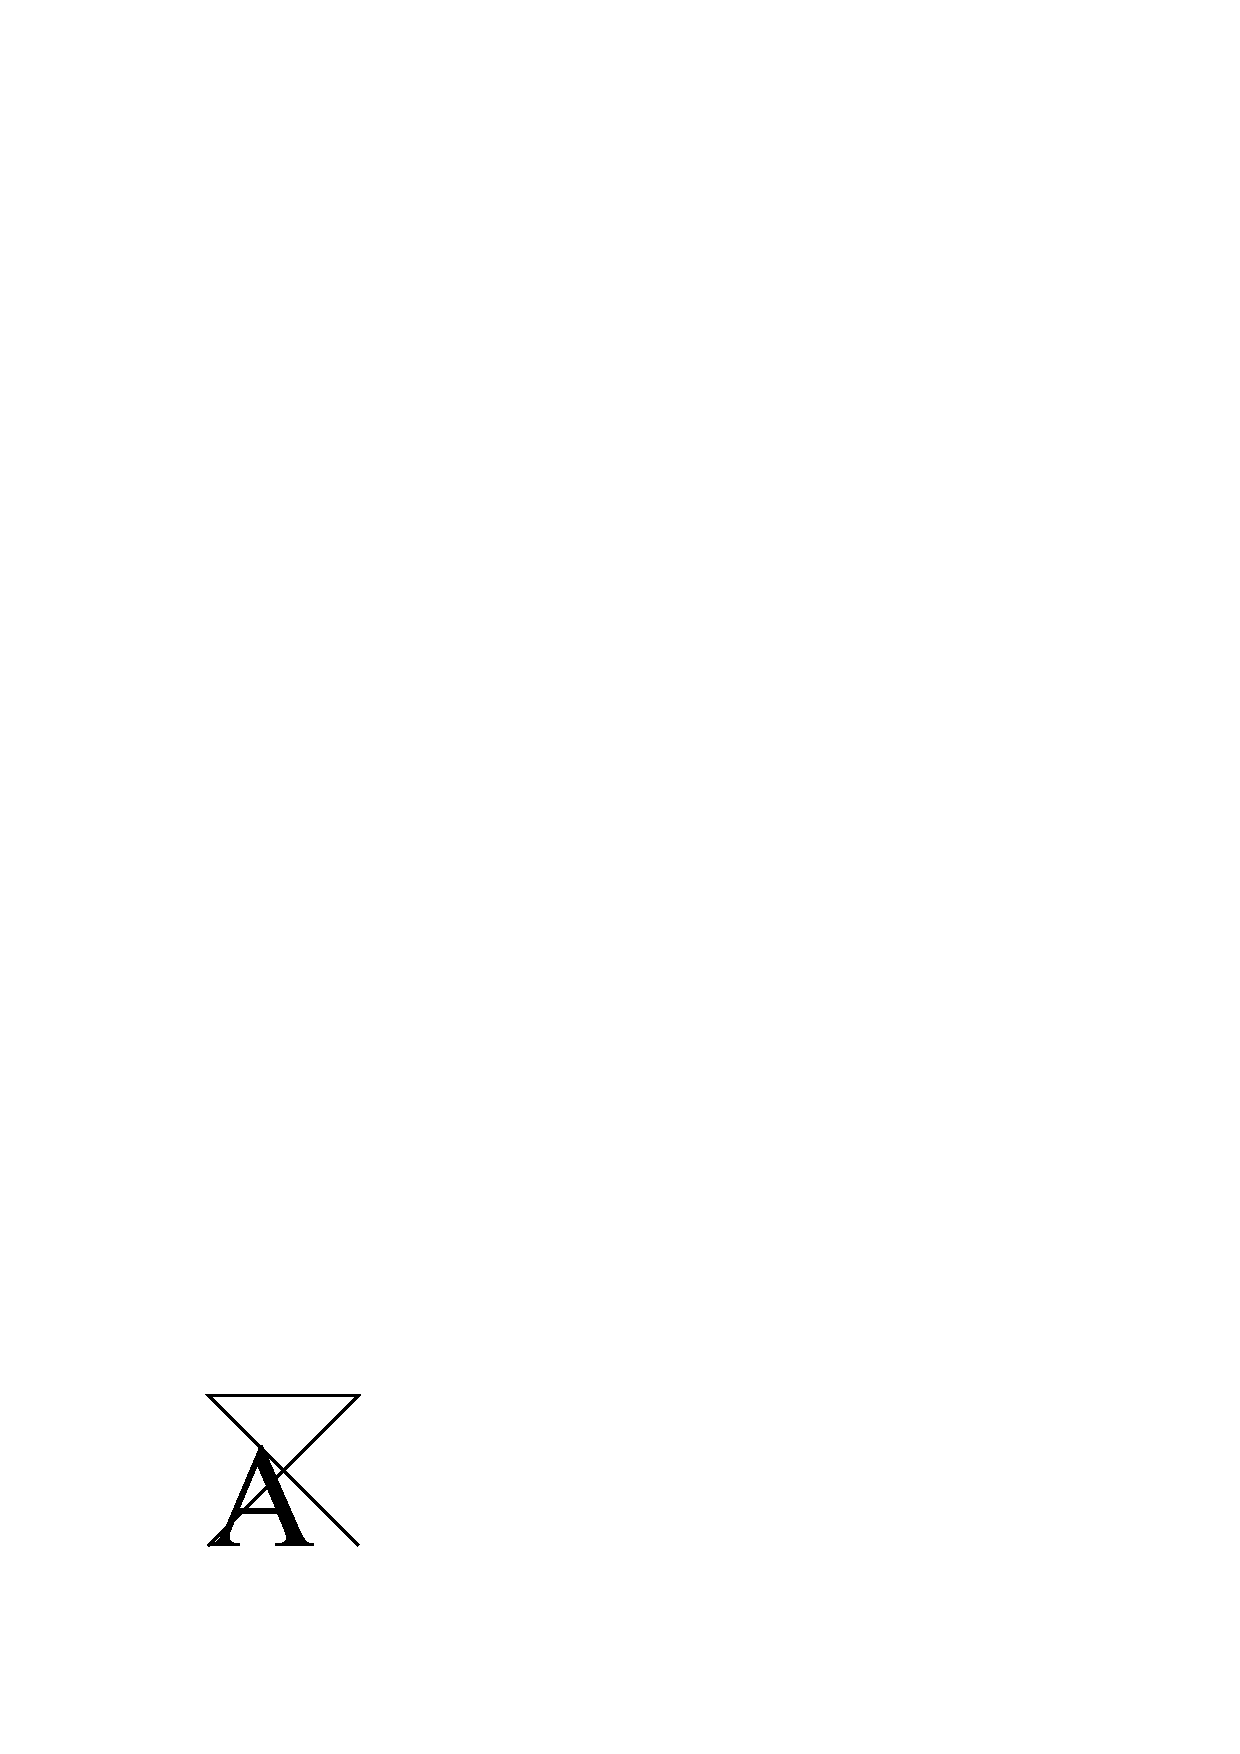
\includegraphics{a} ist ein Bild.
\exb
\begin{verbatim}
Hier 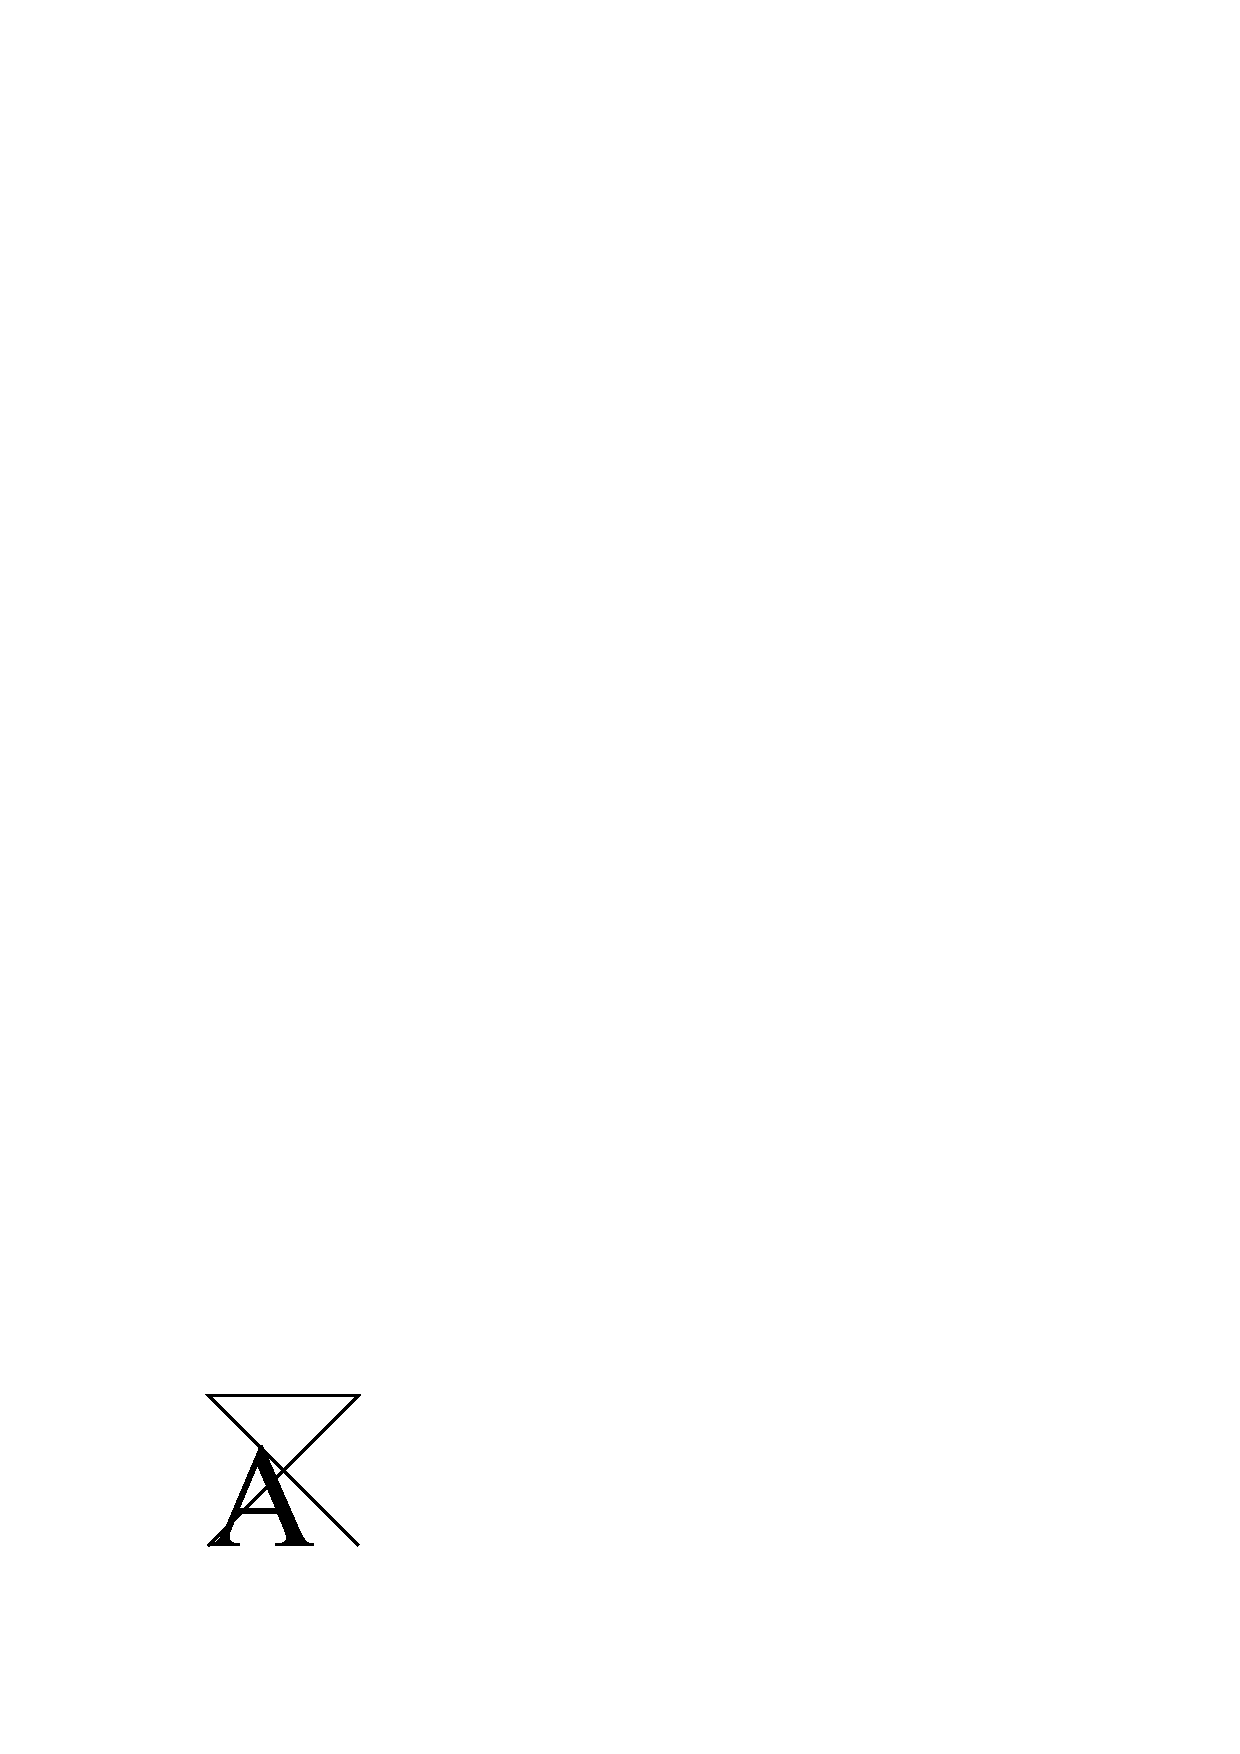
\includegraphics{a} ist
ein Bild
\end{verbatim}
\exc\todo{PG: hier ein schöneres Bild einbinden}
Wird das Paket \texttt{graphicx} mit der Option \texttt{[draft]} geladen,
dann erscheint anstelle des Bildes nur ein Rahmen entsprechend
der tatsächlichen Bildgröße mit dem Namen des Grafikfiles, 
was die Bearbeitung beschleunigt und für Probeausdrucke nützlich ist.

Weitere Informationen zum Einbinden von Bildern finden Sie in der
Online"=Dokumentation \cite{grfguide}, im \textit{Graphics Companion}
\cite{grfcomp} und in K.~Reckdahls empfehlenswertem  Tutorium \cite{epslatex}.




%: Seitenaufbau
\section{Seitenaufbau}

\subsection{Kopf- und Fußzeilen} 
Der Inhalt von Kopf- und  Fußzeilen kann mit dem Befehl
\begin{beispiel}
\verb|\pagestyle{|\textit{style}\verb|}|
\end{beispiel}
festgelegt werden:
 
Mit \verb|\pagestyle{plain}| steht
die Seitennummer zentriert in der Fußzeile; 
das ist die Voreinstellung und braucht normalerweise nicht explizit 
angegeben zu werden.
Mit dem Stil \texttt{headings} stehen Kapitel-Überschrift und
Seitennummer in der Kopfzeile.
Mit \texttt{empty} sind Kopf- und Fußzeile leer.  Der Befehl
\begin{beispiel}
\verb|\thispagestyle{|\textit{style}\verb|}|
\end{beispiel}
gilt entsprechend nur für die aktuelle Seite.  Einige Befehle, wie etwa
\verb|\chapter|, ändern den Stil der aktuellen Seite.  Diese Änderungen 
kann man durch einen nachfolgenden \verb|\thispagestyle|-Befehl aufheben.

Im \manual\ ist angegeben, wie man das Aussehen der Kopf- und Fußzeilen
außerdem mit dem Seitenstil 
\verb|myheadings| und den Befehlen
\verb|\markboth|,
\verb|\markright| und
\verb|\pagenumbering|
beeinflussen kann.

\subsection{Gleitobjekte} \label{floats}
Große Bilder und lange Tabellen lassen sich nicht immer genau 
dort unterbringen, wo sie inhaltlich hingehören, weil sie nicht mehr 
vollständig auf die aktuelle Seite passen, aber auch nicht durch einen 
Seitenwechsel zerrissen werden sollen.  Um  solche Strukturen automatisch
an eine geeignete Stelle "`gleiten"' zu lassen, kennt \LaTeX{} die beiden 
Umgebungen \texttt{figure} und \texttt{table}.  

\subsubsection{Abbildungen (figure)}
Diese Umgebung ist für die Behandlung von Abbildungen gedacht.
Tatsächlich spielt es aber keine Rolle, \emph{wie} diese erzeugt wurden:
Alles, was zwischen
\verb|\begin{figure}| und \verb|\end{figure}|
steht, wird automatisch an eine Stelle
gesetzt, wo es komplett hinpasst, ohne durch einen Seitenwechsel
zerrissen zu werden.  

Mit \verb|\caption{...}| setzt man die Bezeichnung der Abbildung.
Dabei ist nur der Text anzugeben, das Wort "`Abbildung"' und die
fortlaufende Nummer werden von \LaTeX\ hinzugefügt.
Bei Abbildungen ist es allgemein üblich, die Bezeichnung
\emph{unter} das Bild zu setzen.
Mit \verb|\label| und \verb|\ref| kann man die Nummer der
Abbildung im Text ansprechen, mit \verb|\pageref| ihre Seitenzahl.
Der Befehl \verb:\label: muss dabei \emph{nach} dem \verb:\caption:-Befehl
stehen, sonst stimmt die Nummerierung nicht!

Im folgenden Beispiel wird einfach mit dem Befehl \verb|\vspace|
(siehe Abschnitt \ref{vabstaende})
leerer Raum für ein später einzusetzendes Bild gelassen:
\exa
Abbildung~\ref{weiss} auf S.~\pageref{weiss} zeigt ein
Beispiel aus der Minimal art.
\exb
\begin{verbatim}
Abbildung~\ref{weiss} auf
S.~\pageref{weiss} zeigt
ein Beispiel aus der 
Minimal art.
\begin{figure}[tb]
\vspace{6cm}
\caption{Landschaft im
Nebel} \label{weiss}
\end{figure}
\end{verbatim}
\exc
\begin{figure}[tb]
\vspace{6cm}
\caption{Landschaft im
Nebel} \label{weiss}
\end{figure}

\LaTeX\ kann eine Abbildung nach verschiedenen Kriterien platzieren:
\texttt{h} "`here"' (hier),
\texttt{t} "`top"' (oben auf der Seite), \texttt{b} "`bottom"' (unten
auf der Seite) oder \texttt{p} "`page"' (eigene Seite für
Abbildungen).

Die Parameter in den eckigen Klammern, die wahlweise angegeben
werden können, dienen dazu, die Platzierung der Abbildung auf die
angegebenen Orte \emph{einzuschränken}.  Durch Angabe von
z.\,B.\ \texttt{tb}
wird \LaTeX{} angewiesen, nur eine Platzierung oben oder unten auf der
Seite zu versuchen, je nachdem,
wo \emph{zuerst} eine passende Stelle gefunden wird.
Werden keine Parameter (und keine eckigen
Klammern!) angegeben, ist die Voreinstellung \texttt{tbp},
also ohne~\texttt{h}.

Eine Platzierungsbeschränkung \emph{nur} auf \texttt{[h]} ist unsinnig;
sie würde das "`Gleiten"' ja gerade verhindern.
Wenn der Platz "`hier"' nicht ausreicht, 
verschiebt \LaTeX{} dann die Abbildung mindestens 
bis zum Anfang der nächsten Seite, so als hätte man \texttt{[ht]} angegeben.

Eine Abbildung, die nicht platziert werden konnte, wird von
\LaTeX\ immer weiter nach hinten verschoben (und schiebt alle
weiteren Abbildungen vor sich her!), bis ein neues Kapitel
beginnt, das Dokument zu Ende ist, oder der Befehl
\verb|\clearpage| eingegeben wird.  


Es gibt noch einen weiteren Platzierungsparameter, 
\texttt{!} (bang), der \LaTeX{} anweist,
gewisse eingebaute Beschränkungen zu ignorieren, 
z.\,B., dass bei der Platzierung gemäß \texttt{h}, \texttt{t} oder \texttt{b}
ein Mindestanteil der Seite für normalen Text übrig bleiben muss.
"`Bang"' muss immer zusammen mit mindestens einem der vier
anderen Parameter benutzt werden.  
 


\subsubsection{Tabellen (table)}

Damit Tabellen nicht auf einen Seitenwechsel fallen,
können sie, analog zu Abbildungen, zwischen
\verb|\begin{table}| und \verb|\end{table}| gesetzt werden.
Die Befehle
\verb|\caption|, \verb|\label|, \verb|\ref| und \verb|\pageref|
wirken entsprechend.
Hier sind beide möglichen Konventionen verbreitet: Die
Bezeichnung wird entweder immer \emph{über} oder immer
\emph{unter} die Tabelle gesetzt.

Auch hier gilt, dass in der \texttt{table}"=Umgebung  beliebiger
Text stehen darf; die Tabelle muss nicht zwangsläufig durch die
\texttt{tabular}"=Umgebung erzeugt worden sein.
Der Unterschied zu \texttt{figure} besteht nur darin, 
dass die Bezeichnung mit dem Wort "`Tabelle"' versehen wird,
und dass die Tabellen unabhängig von den Abbildungen nummeriert werden.

\endinput

\clearpage
%: Schriften
% master: l2kurz.tex
% l2k5.tex - 5.Teil der LaTeX2e-Kurzbeschreibung v2.3
% 2001-04-10 (WaS)

\section{Schriften}
Normalerweise wählt \LaTeX\ die Größe und den Stil der Schrift
aufgrund der Befehle aus, die die logische Struktur des Textes angeben:
Überschriften, Fußnoten, Hervorhebungen usw.
Im folgenden werden Befehle und Makropakete beschrieben, mit denen
die Schrift auch explizit beeinflusst werden kann.
Ausführlichere Erläuterungen zum Umgang mit Schriften in \LaTeX{}
findet man im \textit{\LaTeX-Begleiter} \cite{wonne}
und in der Online-Dokumentation \cite{fntguide}\todo{PG: wenigstens XeTeX und LuaTeX mit fontspec erwähnen?\\MD: Ich denke, dem sollte ein eigener Abschnitt gewidmet werden.\\PG: die Textlänge...}.



\subsection{Schriftgrößen}
 
Die in der Tabelle~\ref{sizes} angeführten Befehlen 
wechseln die Schriftgröße.
Sie spezifizieren die Größe relativ
zu der von \verb:\documentclass: festgelegten Grundschrift.
Ihr Wirkung reicht bis zum Ende der aktuellen Gruppe oder Umgebung.


\begin{table}[hb]
\caption{Schriftgrößen} \label{sizes}
\begin{lminipage}{10cm}
\begin{tabbing}
\texttt{xfootnotesizexx}\= und dann der Text \kill
\verb|\tiny|         \> \tiny        winzig kleine Schrift \\
\verb|\scriptsize|   \> \scriptsize  sehr kleine Schrift (wie Indizes)\\
\verb|\footnotesize| \> \footnotesize     kleine Schrift (wie Fußnoten)\\
\verb|\small|        \> \small            kleine Schrift \\
\verb|\normalsize|   \> \normalsize  normale Schrift \\
\verb|\large|        \> \large       große Schrift \\
\verb|\Large|        \> \Large       größere Schrift \\
\verb|\LARGE|        \> \LARGE       sehr große Schrift \\[3pt]
\verb|\huge|         \> \huge        riesig groß \\[3pt]
\verb|\Huge|         \> \Huge        gigantisch
\end{tabbing}
\end{lminipage}
\end{table}
 
Die Größen-Befehle verändern auch die Zeilenabstände auf
die jeweils passenden Werte -- aber nur, wenn die
Leerzeile, die den Absatz beendet, innerhalb des
Gültigkeitsbereichs des Größen-Befehls liegt:
\exa
{\Large zu enger\\
Abstand}\par
\exb
\begin{verbatim}
{\Large zu enger \\
Abstand}\par
\end{verbatim}
\exc
\exa
{\Large richtiger\\
Abstand\par}
\exb
\begin{verbatim}
{\Large richtiger\\
Abstand\par}
\end{verbatim}
\exc
Für korrekte
Zeilenabstände darf die
schließende geschwungene Klammer also nicht zu früh kommen,
sondern erst nach einem Absatzende, das übrigens nicht nur als
Leerzeile, sondern auch als Befehl \verb|\par|  eingegeben werden 
kann.


\subsection{Schriftstil}
Der Schriftstil wird in \LaTeX{} durch 3~Merkmale definiert:
\begin{description}
\item[Familie] Standardmäßig stehen 3~Familien zur Wahl:
  "`roman"' (Antiqua), "`sans serif"' (Serifenlose) und "`typewriter"'
  (Schreibmaschinenschrift).
\item[Serie] Die Serie gibt Stärke und Laufweite der
  Schrift an: "`medium"' (normale Schrift), "`boldface extended"'
  (fett und breiter).
\item[Form] Die Form der Buchstaben: "`upright"'
  (aufrecht), "`slanted"' (geneigt), "`italic"' (kursiv),
  "`caps and small caps"' (Kapitälchen).
\end{description}
Tabelle~\ref{fonts} zeigt die Befehle, mit denen diese Attribute 
explizit beeinflusst werden können.  
Die Befehle der Form \verb|\text...| setzen nur ihr Argument im 
gewünschten  Stil.  Zu jedem dieser Befehle ist ein Gegenstück angegeben, 
das von seinem Auf\/treten an bis zum Ende der laufenden Gruppe oder Umgebung 
wirkt.

Zu beachten ist, dass Wörter in Schreibmaschinenschrift nicht automatisch
getrennt werden.\par

\begin{table}[hbp]
\caption{Schriftstile} \label{fonts}
\begin{lminipage}{10cm}
\begin{tabbing}\small
\verb|\textnormal|\{\textit{text}\}\qquad\=\verb|\normalfont|\qquad\=\kill
\verb|\textrm|\{\textit{text}\}         \>\verb|\rmfamily|       \>\textrm{Antiqua}\\
\verb|\textsf|\{\textit{text}\}         \>\verb|\sffamily|       \>\textsf{Serifenlose}\\
\verb|\texttt|\{\textit{text}\}         \>\verb|\ttfamily|       \>\texttt{Maschinenschrift}\\[1ex]
\verb|\textmd|\{\textit{text}\}         \>\verb|\mdseries|       \>\textmd{normal}\\
\verb|\textbf|\{\textit{text}\}         \>\verb|\bfseries|       \>\textbf{fett, breiter laufend}\\[1ex]
\verb|\textup|\{\textit{text}\}         \>\verb|\upshape|        \>\textup{aufrecht}\\
\verb|\textsl|\{\textit{text}\}         \>\verb|\slshape|        \>\textsl{geneigt}\\
\verb|\textit|\{\textit{text}\}         \>\verb|\itshape|        \>\textit{kursiv}\\
\verb|\textsc|\{\textit{text}\}         \>\verb|\scshape|        \>\textsc{Kapitälchen}\\[1ex]
\verb|\textnormal|\{\textit{text}\}     \>\verb|\normalfont|     \>\textnormal{Die Grundschrift des Dokuments}
\end{tabbing}
\end{lminipage}
\end{table}

Die Befehle für Familie, Serie und Form können untereinander und mit den
Größen-Befehlen kombiniert werden;  allerdings muss nicht jede
mögliche Kombination tatsächlich als reale Schrift (Font)
zur Verfügung stehen.
\exa
{\small Die kleinen
\textbf{fetten} Römer
beherrschten }{\large das
ganze große \textit{Italien}.}
\\[6ex]
{\Large\sffamily\slshape plakativ}
\exb
\begin{verbatim}
{\small Die kleinen \textbf{fetten}
Römer
beherrschten }{\large das
ganze große \textit{Italien}.}
{\Large\sffamily\slshape plakativ}
\end{verbatim}
\exc

Je \emph{weniger} verschiedene Schriftarten man verwendet, desto
lesbarer und schöner wird das Schriftstück!


\subsection{Andere Schriftfamilien}
Mit den im vorigen Abschnitt eingeführten Befehlen kann man nicht beeinflussen,
welche Schriftfamilien tatsächlich als Antiqua, Serifenlose und
Maschinenschrift benutzt werden.  \LaTeX{} verwendet als Voreinstellung
die sog.\ Computer-Modern-Schriftfamilien (CM), siehe Tabelle~\ref{families};
der Stil der mathematischen Zeichensätze passt dabei zu CM~Roman.

Will man andere Schriften benutzen, dann ist der einfachste Weg 
das Laden eines Pakets, das eine oder mehrere dieser Schriftfamilien 
komplett ersetzt.
Tabelle~\ref{families} führt einige derartige Pakete auf%,
% die allerdings nicht in jeder \LaTeX-Installation verfügbar sein müssen
.

Die Dokumentation Ihres \TeX-Systems \cite{local} sollte darüber
informieren, welche Schriften verfügbar sind
und wie Sie weitere installieren und verwenden können.
Insbsondere sollte eine Anzahl von verbreiteten PostScript-Schriften
mit jedem aktuellen \LaTeX-System verwendbar sein \cite{postscript}.

\todo[inline]{PG: die Tabelle bekommt sicherlich keinen Schönheitspreis. Lieber mit \cs{toprule},\cs{midrule} und \cs{bottomrule} machen. Außerdem könnten wir die Liste vielleicht auf einen aktuelleren Stand bringen? Siehe \url{http://tex.stackexchange.com/questions/59403}\\MD: JA}

\begin{table}[htb]
\caption[Pakete für alternative Schriftfamilien]
{Pakete für alternative Schriftfamilien (Eine leere
Tabellenspalte bedeutet, dass das Paket die betreffende Schriftfamilie nicht 
verändert; * kennzeichnet die jeweils als Grundschrift eingestellte Familie.)}
\label{families}
{\footnotesize
\begin{center}
\medskip
\renewcommand{\arraystretch}{1.5}
\begin{tabular}{|l|p{2.cm}p{2.2cm}p{2.4cm}p{2.2cm}|}
\hline
Paket            & Antiqua    & Serifenlose   & Schreibmaschine  & math.\ Formeln\\\hline\hline
(keines)         & CM Roman * & CM Sans Serif & CM Typewriter    & $\approx$ CM Roman\\\hline
\texttt{ccfonts} & Concrete *
                 &
                 &
                 & $\approx$ Concrete\\\hline
\texttt{cmbright}&
                 & CM Bright *
                 & {\raggedright CM\ Typewriter\\ Light}
                 & $\approx$ CM Bright\\\hline
% \texttt{pandora} & {\raggedright Pandora\\ Roman *} 
%                  & {\raggedright Pandora \\ Sans Serif} 
%                  &
%                  & \\\hline
\texttt{mathptmx}& Times *
                 &
                 &
                 & $\approx$ Times\\\hline
\texttt{mathpazo}& Palatino *
                 &
                 &
                 & $\approx$ Palatino\\\hline
\texttt{helvet}  & 
                 & Helvetica
                 &
                 & \\\hline
\texttt{courier} &
                 &
                 & Courier 
                 & \\\hline
\end{tabular}
\end{center}
}
\end{table}


\subsection{Die "`europäischen"' Zeichensätze}
\LaTeX{} verwendet standardmäßig  Schriften mit einem Umfang von
128~Zeichen.  Umlaute oder akzentuierte Buchstaben sind darin nicht
enthalten; sie werden jeweils aus dem Grundsymbol und dem Akzent
zusammengesetzt.  

Inzwischen stehen die meisten der mit \LaTeX\ verwendbaren Schriften
auch mit einem erweiterten "`europäischen"' Zeichenvorrat bereit.
Sie enthalten jetzt 256 Zeichen, welche fast
alle europäischen Sprachen abdecken, d.\,h., jedes benötigte
Zeichen ist vorgefertigt in ihnen enthalten.
Das hat nicht nur eine
höhere typographische Qualität zur Folge; aufgrund der inneren Arbeitsweise
von \TeX{} entfallen damit auch die Einschränkungen im Zusammenhang mit
der Silbentrennung, die im Abschnitt~\ref{silb} erwähnt wurden:
Wörter mit Umlauten werden nun besser getrennt, und im Argument des
Befehls \verb|\hyphenation| dürfen auch Umlaute und das scharfe~s stehen.

%% stimmt nur fuer EC
%Weiterhin sind die Unterschneidungen im Vergleich zu den amerikanischen
%\TeX-Originalschriften stark verbessert und nun auch auf häufige
%Buchstabenpaarungen in nicht-englischen Sprachen optimiert.

% <------- Formulierung ????
Die europäischen Schriften bestehen aus zwei Teilen: Der T1-Zeichensatz
enthält Buchstaben, ASCII-Zeichen sowie verschiedene Anführungszeichen
und Striche, 
während ein ergänzender TS1-Zeichensatz zusätzliche Textsymbole bereitstellt.
% <------- Formulierung ????

\LaTeX{} wird veranlasst, T1-Schriften zu verwenden,
indem man das Paket \texttt{fontenc} mit der Option \texttt{T1} lädt:
\begin{quote}
  \verb|\usepackage[T1]{fontenc}|
\end{quote}
Das Paket \texttt{textcomp} ermöglicht den Zugriff auf die Textsymbole:
\begin{quote}
  \verb|\usepackage{textcomp}|
\end{quote}
Welche zusätzlichen Zeichen mit den T1-Schriften
bereitgestellt werden, ist in \cite{usrguide} zusammengefasst;
Anhang~\ref{textsymbols} der vorliegenden Kurzbeschreibung
enthält eine Liste aller TS1-Textsymbole.  Einige der Textsymbole sind
auch ohne das Paket \texttt{textcomp} verfügbar, siehe Abschnitt~\ref{symbole},
dann aber nicht immer in einem zur laufenden Schrift passenden Stil.

Beachten Sie, dass in Fonts, die nicht speziell für die Verwendung 
mit \TeX\ entworfen wurden, 
nur ein Teil der TS1-Textsymbole enthalten ist.
Das betrifft vor allem die "`handelsüblichen"' PostScript-Schriften.

\endinput


\clearpage
%: Spezialitäten
%!TEX root = l2kurz.tex

% master: l2kurz.tex
% l2k6.tex - 6.Teil der LaTeX2e-Kurzbeschreibung v2.3
% 2003-04-10 (WaS)

\section{Spezialitäten}

Das komplette Menü der Spezialitäten, die von \LaTeX\ serviert
werden, ist im \manual\ und in der Online-Dokumentation beschrieben.
Hier soll nur auf einige besondere "`Schmankerln"' hingewiesen
werden.

\subsection{Abstände}

\subsubsection{Zeilenabstand}

Um in einem Schriftstück größere Zeilenabstände zu verwenden,
als es in der Dokumentklasse vorgesehen ist, gibt es in
\LaTeX\ den Befehl \lstinline:\linespread:, der im Vorspann stehen sollte
und dann auf das gesamte Dokument wirkt.  Das kann beispielsweise
dann notwendig werden, wenn eine Schrift benutzt wird, die eine größerer x-Höhe
hat als die voreingestellte Computer-Modern.  Für die Schrift "`Palatino"' etwa
ist eine Vergrößerung des Zeilenabstandes um ca.\ 5\,\% angemessen:
\begin{quote}
\lstinline|\usepackage{mathpazo}|\\
\lstinline|\linespread{1.05}|
\end{quote}

Häufig wird ein anderthalbfacher Zeilenabstand gewünscht, wobei bspw. Fußnoten ausgenommen
sein sollen. Der Befehle \lstinline:\linespread: macht diese Unterscheidung nicht. Zur
Änderung des Zeilenabstandes sollte daher stets auf das Paket \texttt{setspace} zurückgegriffen werden.



\subsubsection{Spezielle horizontale Abstände}\label{abst:horiz}

Die Abstände zwischen Wörtern und Sätzen werden von \LaTeX\
automatisch gesetzt.
Sonstigen horizontalen Abstand kann man mit den Befehlen
\begin{beispiel}
\lstinline|\hspace{|\textit{länge}\lstinline|}|\\
\lstinline|\hspace*{|\textit{länge}\lstinline|}|
\end{beispiel}
einfügen. Wenn der Abstand auch am Beginn oder Ende einer Zeile
erhalten bleiben soll, muss \lstinline|\hspace*| statt \lstinline|\hspace|
geschrieben werden.

Die Längenangabe besteht im einfachsten Fall aus einer Zahl
und einer Einheit.  Die wichtigsten Einheiten sind in
Tabelle~\ref{units} angeführt.
\begin{table}[!htb]
\caption{Einheiten für Längenangaben} \label{units}
\centering
\def\arraystretch{1.25}
\begin{tabular}{@{}ll@{}}
\toprule
\texttt{mm} & Millimeter                               \\
\texttt{cm} & Zentimeter = 10\,mm                            \\
\texttt{in} & inch $= 25.4\,\mathrm{mm} $                 \\
\texttt{pt} & point $ =(1/72.27)\,\mathrm{in}
                        \approx 0.351\,\mathrm{mm}$         \\
\texttt{bp} & big point $ =(1/72)\,\mathrm{in}
                            \approx 0.353\,\mathrm{mm} $     \\
%\texttt{dd} \> Didot-Punkt \( = (1238/1157)\,\mathrm{pt}
%                              \approx 0.376\,\mathrm{mm} \)   \\
% --- wegen unklarer Definition (0.375 ider 0.376mm) besser nicht benutzen!
\texttt{em}  &  Geviert (doppelte Breite einer Ziffer der aktuellen Schrift)\\
\texttt{ex}   & Höhe des Buchstabens x der aktuellen Schrift \\
\bottomrule
\end{tabular}
\end{table}

Die Befehle in Tabelle~\ref{hspace} sind Abkürzungen zum Einfügen
besonderer horizontaler Abstände.

\begin{table}[!htb]
\caption{Befehle für horizontale Abstände} \label{hspace}
\centering
\def\arraystretch{1.25}
\begin{tabular}{@{}ll@{}}
\toprule
\lstinline|\,|       & ein sehr kleiner Abstand (siehe auch Abschnitt~\ref{abstaende})\\
\lstinline|\enspace| & so breit wie eine Ziffer \\
\lstinline|\quad|    & so breit, wie ein Buchstabe hoch ist
                   ("`weißes Quadrat"') \\
\lstinline|\qquad|   & doppelt so breit wie ein \lstinline|\quad| \\
\lstinline|\hfill|   & ein Abstand, der sich von 0 bis \(\infty\)
                   ausdehnen kann. \\
\bottomrule
\end{tabular}
\end{table}

Der Befehl \lstinline|\hfill|  kann dazu dienen, einen vorgegebenen Platz auszufüllen.

\begin{LTXexample}
\raggedright
Schafft mir\hspace{1.5cm}Raum! \\
$\triangleleft$\hfill
$\triangleright$
\end{LTXexample}



\subsubsection{Spezielle vertikale Abstände} \label{vabstaende}

Die Abstände zwischen Absätzen, Kapiteln usw.\ werden von
\LaTeX\ automatisch bestimmt.
In Spezialfällen kann man zusätzlichen Abstand
\emph{zwischen zwei Absätzen} mit dem Befehl
\begin{beispiel}
\lstinline|\vspace{|\textit{länge}\lstinline|}|
\end{beispiel}
bewirken.
Dieser Befehl sollte immer zwischen zwei Leerzeilen angegeben
werden.
Wenn der Abstand auch am Beginn oder Ende einer Seite erhalten
bleiben soll, muss \lstinline|\vspace*| statt \lstinline|\vspace|
geschrieben werden.
Die Befehle in Tabelle~\ref{vspace} sind Abkürzungen für
bestimmte vertikale Abstände.
\begin{table}[!htb]
\caption{Befehle für vertikale Abstände} \label{vspace}
\centering
\def\arraystretch{1.25}
\begin{tabular}{@{}ll@{}}
\toprule
\lstinline|\smallskip| & etwa $\nfrac{1}{4}$ Zeile \\
\lstinline|\medskip|   & etwa $\nfrac{1}{2}$ Zeile \\
\lstinline|\bigskip|   & etwa 1 Zeile \\
\lstinline|\vfill|     & ein Abstand, der sich von 0 bis $\infty$
                     ausdehnen kann\\
\bottomrule
\end{tabular}
\end{table}

Der Befehl \lstinline|\vfill| in Verbindung mit \lstinline|\newpage|
kann dazu dienen, Text an den unteren Rand einer Seite zu setzen
oder vertikal zu zentrieren.  Beispielsweise enthält der Quelltext
für die zweite Seite der vorliegenden Beschreibung:
\clearpage
\begin{example}
\vfill

Dieses Dokument wurde mit \LaTeX{} gesetzt.
...
\newpage
\end{example}


Zusätzlichen Abstand zwischen zwei Zeilen \emph{innerhalb}
eines Absatzes oder einer Tabelle erreicht man mit dem Befehl
\lstinline|\\[|\textit{länge}\lstinline|]|.

\begin{LTXexample}
Albano Cesara \\
Lindenallee 10 \\[1.5ex]
95632 Pestitz
\end{LTXexample}


% \subsection{\LaTeX-Zeichenprogramme}

% \todo[inline]{PG: hier eine kurze Erwähnung von TikZ und anschließend ein Bild, ohne große Erklärung? Hast du ein griffiges Beispiel oder sollen wir auf tex.sx nach einem fragen? Mehr als eine Seite würde ich auf keinen Fall damit verbrauchen, lieber mit einer Aufzählung, welche Vorteile sowas hat (Schriftart/Farben wie im Dokument, Grafik und Quelle sind beieinander, oftmals genauer als Zeichenprogramme, Verbindungen mit dem Text möglich) - aber auch hier Nachteil: Einarbeitung}



\subsection{Literaturangaben}

Mit der \texttt{thebibliography}-Umgebung kann man ein
Literaturverzeichnis erzeugen.
Darin beginnt jede Literaturangabe mit \lstinline|\bibitem|.
Als Parameter wird ein Name vereinbart, unter dem die
Literaturstelle im Text zitiert werden kann, und
dann folgt der Text der Literaturangabe.
Die Nummerierung erfolgt automatisch.
Der Parameter bei \lstinline|\begin{thebibliography}| gibt die
maximale Breite dieser Nummernangabe an, also z.\,B.\
\lstinline|{99}| für maximal zweistellige Nummern.

Im Text zitiert man die Literaturstelle dann mit dem Befehl \lstinline|\cite|
und dem vereinbarten Namen als Argument.

\let\origcite\cite
\begin{LTXexample}[preset=\let\cite\origcite]
Partl~\cite{pa} hat
vorgeschlagen ...

\begin{thebibliography}{99}
\bibitem{pa}
H.~Partl: \textit{German \TeX,}
TUGboat Vol.~9, No.~1 (1988)
\end{thebibliography}
\end{LTXexample}

Werden viele Literatureinträge zitiert bzw. verwendet, bietet sich die Nutzung
einer Datenbank an. Die Datenbank besitzt ihre eigene Syntax,
um die benötigten Literatureinträge zu verwalten. Für die komfortable Verwaltung
von Literaturdatenbanken existieren viele Programme wie beispielsweise JabRef (frei) oder
Endnote (kommerziell). Die Datenbank ist im eigentlichen Sinne eine Textdatei mit
Endung \lstinline|bib|.


Für die Verarbeitung dieser Literaturdatenbanken bieten sich zwei verschiedene
Hilfsmittel für \LaTeX{} an. Die klassische Variante ist \emph{Bib\TeX} in Verbindung
mit einem Literaturverzeichnisstil. Die Anpassung an die eigenen Bedürfnisse
gestaltet sich mehr als schwierig. Daher wurde in den letzten Jahren das \LaTeX{}
Makropaket \emph{biblatex} entwickelt, das alternativ zu \emph{Bib\TeX} das mächtigere
Programm \emph{biber} nutzen kann. Das Makropaket \emph{biblatex} erlaubt die Manipulation
des Literaturverzeichnisses auf \LaTeX"=Ebene. Auf CTAN ist eine deutsche Übersetzung der Dokumentation
verfügbar \cite{biblatex-de}.

\endinput

\clearpage
%: Anhang
%!TEX root = l2kurz.tex

% master: l2kurz.tex
% L2KA.TEX - Anhang der LaTeX-Kurzbeschreibung v2.2
% 2001-06-08 (WaS)

\appendix
%\settocdepth{1}

\enlargethispage*{2.5\baselineskip}

\section{Mit dem Paket \texttt{textcomp} verfügbare Symbole}
\label{textsymbols}
{\small
\begin{tabbing}
\quad\quad\=\texttt{Mtextquotestraightdblbase}\hspace{1cm}\=\quad\quad\=\kill
\textquotestraightbase \> \lstinline+\textquotestraightbase+\textsuperscript{*}  \> \textquotestraightdblbase \> \lstinline+\textquotestraightdblbase+\textsuperscript{*} \\
\texttwelveudash \> \lstinline+\texttwelveudash+\textsuperscript{*}  \> \textthreequartersemdash \> \lstinline+\textthreequartersemdash+\textsuperscript{*} \\
\textleftarrow \> \lstinline+\textleftarrow+ \> \textrightarrow \> \lstinline+\textrightarrow+\\
\textblank \> \lstinline+\textblank+ \> \textdollar \> \lstinline+\$+\textsuperscript{*} \\
\textquotesingle \> \lstinline+\textquotesingle+\textsuperscript{*}  \> \textasteriskcentered \> \lstinline+\textasteriskcentered+\textsuperscript{*} \\
\textdblhyphen \> \lstinline+\textdblhyphen+ \> \textfractionsolidus \> \lstinline+\textfractionsolidus+\textsuperscript{*} \\
\textlangle \> \lstinline+\textlangle+ \> \textminus \> \lstinline+\textminus+\textsuperscript{*} \\
\textrangle \> \lstinline+\textrangle+ \> \textmho \> \lstinline+\textmho+\\
\textbigcircle \> \lstinline+\textbigcircle+ \> \textohm \> \lstinline+\textohm+\\
\textlbrackdbl \> \lstinline+\textlbrackdbl+ \> \textrbrackdbl \> \lstinline+\textrbrackdbl+\\
\textuparrow \> \lstinline+\textuparrow+ \> \textdownarrow \> \lstinline+\textdownarrow+\\
\textasciigrave \> \lstinline+\textasciigrave+\textsuperscript{*}  \> \textborn \> \lstinline+\textborn+\\
\textdivorced \> \lstinline+\textdivorced+ \> \textdied \> \lstinline+\textdied+\\
\textleaf \> \lstinline+\textleaf+ \> \textmarried \> \lstinline+\textmarried+\\
\textmusicalnote \> \lstinline+\textmusicalnote+ \> \texttildelow \> \lstinline+\texttildelow+\textsuperscript{*} \\
\textdblhyphenchar \> \lstinline+\textdblhyphenchar+ \> \textasciibreve \> \lstinline+\textasciibreve+\textsuperscript{*} \\
\textasciicaron \> \lstinline+\textasciicaron+\textsuperscript{*}  \> \textacutedbl \> \lstinline+\textacutedbl+\textsuperscript{*} \\
\textgravedbl \> \lstinline+\textgravedbl+\textsuperscript{*}  \> \textdagger \> \lstinline+\dag+\textsuperscript{*} \\
\textdaggerdbl \> \lstinline+\ddag+\textsuperscript{*} \> \textbardbl \> \lstinline+\textbardbl+\textsuperscript{*} \\
\textperthousand \> \lstinline+\textperthousand+\textsuperscript{*} \> \textbullet \> \lstinline+\textbullet+\textsuperscript{*} \\
\textcelsius \> \lstinline+\textcelsius+\textsuperscript{*}  \> \textdollaroldstyle \> \lstinline+\textdollaroldstyle+\\
\textcentoldstyle \> \lstinline+\textcentoldstyle+ \> \textflorin \> \lstinline+\textflorin+\textsuperscript{*} \\
\textcolonmonetary \> \lstinline+\textcolonmonetary+ \> \textwon \> \lstinline+\textwon+\\
\textnaira \> \lstinline+\textnaira+ \> \textguarani \> \lstinline+\textguarani+\\
\textpeso \> \lstinline+\textpeso+ \> \textlira \> \lstinline+\textlira+\\
\textrecipe \> \lstinline+\textrecipe+ \> \textinterrobang \> \lstinline+\textinterrobang+\\
\textinterrobangdown \> \lstinline+\textinterrobangdown+ \> \textdong \> \lstinline+\textdong+\\
\texttrademark \> \lstinline+\texttrademark+\textsuperscript{*} \> \textpertenthousand \> \lstinline+\textpertenthousand+\\
\textpilcrow \> \lstinline+\textpilcrow+ \> \textbaht \> \lstinline+\textbaht+\\
\textnumero \> \lstinline+\textnumero+ \> \textdiscount \> \lstinline+\textdiscount+\\
\textestimated \> \lstinline+\textestimated+ \> \textopenbullet \> \lstinline+\textopenbullet+\\
\textservicemark \> \lstinline+\textservicemark+ \> \textlquill \> \lstinline+\textlquill+\\
\textrquill \> \lstinline+\textrquill+ \> \textcent \> \lstinline+\textcent+\textsuperscript{*} \\
\textsterling \> \lstinline+\pounds+\textsuperscript{*}  \> \textcurrency \> \lstinline+\textcurrency+\textsuperscript{*} \\
\textyen \> \lstinline+\textyen+\textsuperscript{*} \> \textbrokenbar \> \lstinline+\textbrokenbar+\textsuperscript{*} \\
\textsection \> \lstinline+\S+\textsuperscript{*}  \> \textasciidieresis \> \lstinline+\textasciidieresis+\textsuperscript{*} \\
\textcopyright \> \lstinline+\copyright+\textsuperscript{*} \> \textordfeminine \> \lstinline+\textordfeminine+\textsuperscript{*} \\
\textcopyleft \> \lstinline+\textcopyleft+ \> \textlnot \> \lstinline+\textlnot+\textsuperscript{*} \\
\textcircledP \> \lstinline+\textcircledP+ \> \textregistered \> \lstinline+\textregistered+\textsuperscript{*} \\
\textasciimacron \> \lstinline+\textasciimacron+\textsuperscript{*}  \> \textdegree \> \lstinline+\textdegree+\textsuperscript{*} \\
\textpm \> \lstinline+\textpm+\textsuperscript{*} \> \texttwosuperior \> \lstinline+\texttwosuperior+\\
\textthreesuperior \> \lstinline+\textthreesuperior+ \> \textasciiacute \> \lstinline+\textasciiacute+\textsuperscript{*} \\
\textmu \> \lstinline+\textmu+\textsuperscript{*} \> \textparagraph \> \lstinline+\P+\textsuperscript{*} \\
\textperiodcentered \> \lstinline+\textperiodcentered+\textsuperscript{*} \> \textreferencemark \> \lstinline+\textreferencemark+\\
\textonesuperior \> \lstinline+\textonesuperior+ \> \textordmasculine \> \lstinline+\textordmasculine+\textsuperscript{*} \\
\textsurd \> \lstinline+\textsurd+ \> \textonequarter \> \lstinline+\textonequarter+\\
\textonehalf \> \lstinline+\textonehalf+ \> \textthreequarters \> \lstinline+\textthreequarters+\\
\textsf{\texteuro} \> \lstinline+\textsf{\texteuro}+ \> \texttimes \> \lstinline+\texttimes+\textsuperscript{*} \\
\textdiv \> \lstinline+\textdiv+\textsuperscript{*} \\
\end{tabbing}
}

{\footnotesize\noindent 
Schriften, die nicht speziell für die Verwendung mit
\TeX{} entworfen wurden, enthalten normalerweise nur die mit * markierten Zeichen.
\par}

% master: l2kurz.tex
% L2KSYM.TEX - Tabellen zum 3.Teil der LaTeX2e-Kurzbeschreibung v2.0, Erlangen 1998
% L2KSYM.TEX - Tabellen zum 3.Teil der LaTeX2e-Kurzbeschreibung Mainz 1994, 1995
% LKSYM.TEX  - Tabellen zum 3.Teil der LaTeX-Kurzbeschreibung Graz-Wien 1987
% last changes: 1999-09-01 WaS

\subsection{Liste der mathematischen Symbole}  \label{symbols}

In den folgenden Tabellen sind alle Symbole angeführt, die
standardmäßig im mathematischen Modus verwendet werden
können.  Die mit * versehenen Symbole werden
in \LaTeXe\ nur durch das Paket \texttt{latexsym} bereitgestellt.  Bei
vielen Installationen stehen mit den Paketen \texttt{amssymb}, 
\texttt{mathrsfs} oder \texttt{wasysym} weitere Zeichen zur 
Verfügung, näheres steht im \local.
\todo{MD: Wenn solche Übersichten generiert werden, sollte sie m.E. in den Anhang.\\PG: ja, gute Idee.}

\begin{table}[hbp]
\caption{Mathematische Akzente}  \label{mathakz}
\begin{symbols}
$\hat a$    \> \verb|\hat a|   \> $\dot a$   \> \verb|\dot a|   \> $\check a$    \> \verb|\check a|    \\ 
$\tilde a$  \> \verb|\tilde a| \> $\ddot a$  \> \verb|\ddot a|  \> $\breve a$    \> \verb|\breve a|    \\
$\vec a$    \> \verb|\vec a  | \> $\acute a$ \> \verb|\acute a| \> $\mathring a$ \> \verb|\mathring a| \\
$\bar a$    \> \verb|\bar a|   \> $\grave a$ \> \verb|\grave a| \\
\end{symbols}
\end{table}

 
\begin{table}[!htbp]
\caption{Kleine griechische Buchstaben}
\begin{symbols}
$\alpha$   \> \verb|\alpha|    \>$\iota $  \> \verb|\iota|
  \>$\varrho$  \> \verb|\varrho| \\
$\beta$    \> \verb|\beta|     \>$\kappa $ \> \verb|\kappa|
  \>$\sigma$   \> \verb|\sigma| \\
$\gamma$   \> \verb|\gamma|    \>$\lambda $\> \verb|\lambda|
  \>$\varsigma$\> \verb|\varsigma| \\
$\delta$   \> \verb|\delta|    \>$\mu $    \> \verb|\mu|
  \>$\tau $    \> \verb|\tau| \\
$\epsilon$ \> \verb|\epsilon|  \>$\nu $    \> \verb|\nu|
  \>$\upsilon$ \> \verb|\upsilon| \\
$\varepsilon$\> \verb|\varepsilon| \>$\xi $\> \verb|\xi|
  \>$\phi$     \> \verb|\phi| \\
$\zeta$    \> \verb|\zeta|     \>$o $      \> \verb|o|
  \>$\varphi $ \> \verb|\varphi| \\
$\eta$     \> \verb|\eta|      \>$\pi $    \> \verb|\pi|
  \>$\chi $    \> \verb|\chi| \\
$\theta$   \> \verb|\theta|    \>$\varpi $ \> \verb|\varpi|
  \>$\psi$     \> \verb|\psi| \\
$\vartheta$\> \verb|\vartheta| \>$\rho $   \> \verb|\rho|
  \>$\omega$   \> \verb|\omega| \\
\end{symbols}
\end{table}
 
 
\begin{table}[htbp]
\caption{Große griechische Buchstaben}
\begin{symbols}
$\Gamma$ \> \verb|\Gamma|  \>$\Xi$     \> \verb|\Xi|
  \>$\Phi$   \> \verb|\Phi| \\
$\Delta$ \> \verb|\Delta|  \>$\Pi$     \> \verb|\Pi|
  \>$\Psi$   \> \verb|\Psi| \\
$\Theta$ \> \verb|\Theta|  \>$\Sigma$  \> \verb|\Sigma|
  \>$\Omega$ \> \verb|\Omega| \\
$\Lambda$\> \verb|\Lambda| \>$\Upsilon$\> \verb|\Upsilon| \\
\end{symbols}
\end{table}


\begin{table}[!htbp]
\caption[Verschiedene sonstige Symbole]%
        {Verschiedene sonstige Symbole
         (* benötigt Paket \texttt{latexsym})}
\begin{symbols}
$\aleph $\> \verb|\aleph| \>$\prime $\> \verb|\prime| \>
$\forall $\> \verb|\forall|  \\
$\hbar $\> \verb|\hbar| \>$\emptyset $\> \verb|\emptyset| \>
$\exists $\> \verb|\exists|  \\
$\imath $\> \verb|\imath| \>$\nabla $\> \verb|\nabla| \>
$\neg $\> \verb|\neg|  \\
$\jmath $\> \verb|\jmath| \>$\surd $\> \verb|\surd| \>
$\flat $\> \verb|\flat| \\
$\ell $\> \verb|\ell| \>$\top $\> \verb|\top| \>
$\natural $\> \verb|\natural| \\
$\wp $\> \verb|\wp| \>$\bot $\> \verb|\bot| \>$\sharp $\> \verb|\sharp| \\
$\Re $\> \verb|\Re| \>$\Diamond $\> \verb|\Diamond|\textsuperscript{*} \>$\clubsuit $\> \verb|\clubsuit| \\
$\Im $\> \verb|\Im| \>$\Box $\> \verb|\Box|\textsuperscript{*} \>$\diamondsuit $\>
\verb|\diamondsuit| \\
$\partial $\> \verb|\partial| \>$\triangle $\> \verb|\triangle| \>
$\heartsuit $\> \verb|\heartsuit| \\
$\infty $\> \verb|\infty| \>$\angle $\> \verb|\angle| \>
$\spadesuit $\> \verb|\spadesuit| \\
$\mho $\> \verb|\mho|\textsuperscript{*} \\
\end{symbols}
\end{table}


\begin{table}[!htbp]
\caption{"`Große"' Operatoren}
\begin{trivlist}\item
\begin{tabular}{@{}ccl@{\qquad}cll@{\qquad}ccl@{}}
$\sum$     & $\displaystyle \sum$    & \verb|\sum|
  & $\bigcap$    & $\displaystyle\bigcap$    & \verb|\bigcap|
  & $\bigodot$   & $\displaystyle\bigodot$   & \verb|\bigodot| \\[6pt]
$\prod$    & $\displaystyle\prod$    & \verb|\prod|
  & $\bigcup$    & $\displaystyle\bigcup$    & \verb|\bigcup|
  & $\bigotimes$ & $\displaystyle\bigotimes$ & \verb|\bigotimes| \\[6pt]
$\coprod$  & $\displaystyle\coprod$  & \verb|\coprod|
  & $\bigsqcup$  & $\displaystyle\bigsqcup$  & \verb|\bigsqcup|
  & $\bigoplus$  & $\displaystyle\bigoplus$  & \verb|\bigoplus| \\[6pt]
$\int$     & $\displaystyle\int$     & \verb|\int|
  & $\bigvee$    & $\displaystyle\bigvee$    & \verb|\bigvee|
  & $\biguplus$  & $\displaystyle\biguplus$  & \verb|\biguplus| \\[6pt]
$\oint$    & $\displaystyle\oint$    & \verb|\oint|
  & $\bigwedge$  & $\displaystyle\bigwedge$  & \verb|\bigwedge|
\end{tabular}
\end{trivlist}
\end{table}


\begin{table}[!htbp]
\caption[Binäre Operatoren]{Binäre Operatoren 
  (* benötigt Paket \texttt{latexsym})}
\begin{symbols}
$+$   \> \verb|+|   \>$-$    \> \verb|-| \> $\div $\> \verb|\div| \\
$\pm $\> \verb|\pm| \>$\cap $\> \verb|\cap| \>$\vee $\> \verb|\vee| \\
$\mp $\> \verb|\mp| \>$\cup $\> \verb|\cup| \>$\wedge $\> \verb|\wedge| \\
$\setminus $\> \verb|\setminus| \>$\uplus $\> \verb|\uplus| \>
$\oplus $\> \verb|\oplus| \\
$\cdot $\> \verb|\cdot| \>$\sqcap $\> \verb|\sqcap| \>
$\ominus $\> \verb|\ominus| \\
$\times $\> \verb|\times| \>$\sqcup $\> \verb|\sqcup| \>
$\otimes $\> \verb|\otimes| \\
$\ast $\> \verb|\ast| \>$\triangleleft $\> \verb|\triangleleft| \>
$\oslash $\> \verb|\oslash| \\
$\star $\> \verb|\star| \>$\triangleright $\> \verb|\triangleright| \>
$\odot $\> \verb|\odot| \\
$\diamond $\> \verb|\diamond| \>$\lhd $\> \verb|\lhd|\textsuperscript{*} \>
$\dagger $\> \verb|\dagger| \\
$\circ $\> \verb|\circ| \>$\rhd $\> \verb|\rhd|\textsuperscript{*} \>
$\ddagger $\> \verb|\ddagger| \\
$\bullet $\> \verb|\bullet| \>$\unlhd $\> \verb|\unlhd|\textsuperscript{*} \>
$\amalg $\> \verb|\amalg| \\
$\bigcirc $\> \verb|\bigcirc| \> $\unrhd$ \> \verb|\unrhd|\textsuperscript{*} \> 
$\wr$ \> \verb|\wr| \\
$\bigtriangleup$ \>\verb|\bigtriangleup| \>
$\bigtriangledown$ \> \verb|\bigtriangledown|\>\\
\end{symbols}
\end{table}


\begin{table}[!htbp]
\caption[Relationen]%
        {Relationen (* benötigt Paket \texttt{latexsym})}
\begin{symbols}
$< $\> \verb|<| \>$>$\> \verb|>| \>$=$\> \verb|=| \\
$\leq $\> \verb|\leq| \>$\geq $\> \verb|\geq| \>$\equiv $\> \verb|\equiv| \\
$\prec $\> \verb|\prec| \>$\succ $\> \verb|\succ| \>$\sim $\> \verb|\sim| \\
$\preceq $\> \verb|\preceq| \>$\succeq $\> \verb|\succeq| \>
$\simeq $\> \verb|\simeq| \\
$\ll $\> \verb|\ll| \>$\gg $\> \verb|\gg| \>$\asymp $\> \verb|\asymp| \\
$\subset $\> \verb|\subset| \>$\supset $\> \verb|\supset| \>
$\approx $\> \verb|\approx| \\
$\subseteq $\> \verb|\subseteq| \>$\supseteq $\> \verb|\supseteq| \>
$\cong $\> \verb|\cong| \\
$\sqsubseteq $\> \verb|\sqsubseteq| \>$\sqsupseteq $\> \verb|\sqsupseteq| \>
$\bowtie $\> \verb|\bowtie| \\
$\sqsubset$ \> \verb|sqsubset|\textsuperscript{*}\>
$\sqsupset$ \> \verb|sqsupset|\textsuperscript{*}\>
$\Join$\> \verb|\Join|\textsuperscript{*} \\
$\in $\> \verb|\in| \>$\ni $\> \verb|\ni| \>
$\notin$ \> \verb|\notin| \\
$\vdash $\> \verb|\vdash| \>$\dashv $\> \verb|\dashv| \>
$\models $\> \verb|\models| \\
$\smile $\> \verb|\smile| \>$\mid $\> \verb|\mid| \>
$\doteq $\> \verb|\doteq| \\
$\frown $\> \verb|\frown| \>$\parallel $\> \verb|\parallel| \>
$\perp $\> \verb|\perp| \\
$:$ \> \verb|:| \> $\propto$ \> \verb|\propto| \\
\end{symbols}
\end{table}

\begin{table}[!htbp]
\caption{Negierte Relationen}
\begin{symbols}
$\not< $\> \verb|\not<| \>$\not> $\> \verb|\not>| \>$\not= $\> \verb|\not=| \\
$\not\leq $\> \verb|\not\leq| \>$\not\geq $\> \verb|\not\geq| \>
  $\not\equiv $\> \verb|\not\equiv| \\
$\not\prec $\> \verb|\not\prec| \>$\not\succ $\> \verb|\not\succ| \>
  $\not\sim $\> \verb|\not\sim| \\
$\not\preceq $\> \verb|\not\preceq| \>$\not\succeq $\> \verb|\not\succeq| \>
  $\not\simeq $\> \verb|\not\simeq| \\
$\not\subset $\> \verb|\not\subset| \>$\not\supset $\> \verb|\not\supset| \>
  $\not\approx $\> \verb|\not\approx| \\
$\not\subseteq $\> \verb|\not\subseteq| \>$\not\supseteq $\>
\verb|\not\supseteq| \>
  $\not\cong $\> \verb|\not\cong| \\
$\not\sqsubseteq $\> \verb|\not\sqsubseteq| \>$\not\sqsupseteq $\>
\verb|\not\sqsupseteq| \>
  $\not\asymp $\> \verb|\not\asymp| \\
\end{symbols}
\end{table}


\begin{table}[!htbp]
\caption[Pfeile]%
        {Pfeile
         (Vertikale Pfeile werden als Klammerungssymbole behandelt, 
         alle anderen als Relationen.
         * benötigt Paket \texttt{latexsym}.)}
\begin{symbols}
$\leftarrow $\> \verb|\leftarrow| \>$\longleftarrow $\>
\verb|\longleftarrow| \>
  $\uparrow $\> \verb|\uparrow| \\
$\Leftarrow $\> \verb|\Leftarrow| \>$\Longleftarrow $\>
\verb|\Longleftarrow| \>
  $\Uparrow $\> \verb|\Uparrow| \\
$\rightarrow $\> \verb|\rightarrow| \>$\longrightarrow $\>
\verb|\longrightarrow| \>
  $\downarrow $\> \verb|\downarrow| \\
$\Rightarrow $\> \verb|\Rightarrow| \>$\Longrightarrow $\>
\verb|\Longrightarrow| \>
  $\Downarrow $\> \verb|\Downarrow| \\
$\leftrightarrow $\> \verb|\leftrightarrow| \>$\longleftrightarrow $\>
\verb|\longleft...| \>
  $\updownarrow $\> \verb|\updownarrow| \\
$\Leftrightarrow $\> \verb|\Leftrightarrow| \>$\Longleftrightarrow $\>
\verb|\Longleft...| \>
  $\Updownarrow $\> \verb|\Updownarrow| \\
$\mapsto $\> \verb|\mapsto| \>$\longmapsto $\> \verb|\longmapsto| \>
  $\nearrow $\> \verb|\nearrow| \\
$\hookleftarrow $\> \verb|\hookleftarrow| \>$\hookrightarrow $\>
\verb|\hookrightarrow| \>
  $\searrow $\> \verb|\searrow| \\
$\leftharpoonup $\> \verb|\leftharpoonup| \>$\rightharpoonup $\>
\verb|\rightharpoonup| \>
  $\swarrow $\> \verb|\swarrow| \\
$\leftharpoondown $\> \verb|\leftharpoondown| \>$\rightharpoondown $\>
\verb|\right...| \>
  $\nwarrow $\> \verb|\nwarrow| \\
$\rightleftharpoons $\> \verb|\rightleftharpoons| \>\>\>
  $\leadsto $\> \verb|\leadsto|\textsuperscript{*} \\
\end{symbols}
\end{table}


\begin{table}[!htbp]
  \caption{Klammern}
\begin{tabbing}
 \hspace{7mm}\=\hspace{2.25cm}\= \hspace{7mm}\=\hspace{3.25cm}\=
 \hspace{7mm}\=\hspace{2.25cm}\= \hspace{7mm}\=\hspace{2.25cm}\=\kill
$($       \> \verb|(|       \> $)$       \> \verb|)| \>
  $\lceil $ \> \verb|\lceil|  \> $\rceil $\> \verb|\rceil| \\
$\langle $\> \verb|\langle| \> $\rangle $\> \verb|\rangle| \>
  $\lfloor $\> \verb|\lfloor| \> $\rfloor $\> \verb|\rfloor| \\
$[$       \> \verb|[|       \> $]$      \>  \verb|]| \>
  $\{$      \> \verb|\{|      \> $\}$     \> \verb|\}| \\
%$\lbrack $\> \verb|\lbrack| \> $\rbrack $\> \verb|\rbrack| \>
%  $\lbrace $\> \verb|\lbrace| \> $\rbrace $\> \verb|\rbrace| \\
$|$       \> \verb.|.       \> $\|$       \> \verb.\|. \>
  $\backslash$ \> \verb.\backslash. \\
\end{tabbing}
\end{table}

\iffalse % In einer Kurz(!)anleitung unnoetig
\begin{table}[!htbp]
\caption{Synonyme}
\bigskip
Für manche Symbole stehen mehrere verschiedene Befehle zur
Verfügung.
\begin{symbols}
\>\>  $\ne $\> \verb|\ne| oder \verb|\neq| \> \verb|\not=| \\
\>\>  $\le $\> \verb|\le| \> \verb|\leq| \\
\>\>  $\ge $\> \verb|\ge| \> \verb|\geq| \\
\>\>  $\{ $\> \verb|\{| \> \verb|\lbrace| \\
\>\>  $\} $\> \verb|\}| \> \verb|\rbrace|  \\
\>\>  $\to $\> \verb|\to| \> \verb|\rightarrow|  \\
\>\>  $\gets $\> \verb|\gets| \> \verb|\leftarrow|  \\
\>\>  $\owns $\> \verb|\owns| \> \verb|\ni|  \\
\>\>  $\land $\> \verb|\land| \> \verb|\wedge|  \\
\>\>  $\lor $\> \verb|\lor| \> \verb|\vee|  \\
\>\>  $\lnot $\> \verb|\lnot| \> \verb|\neg|  \\
\>\>  $\vert $\> \verb|\vert| \> \verb.|.  \\
\>\>  $\Vert $\> \verb|\Vert| \> \verb.\|.  \\
\end{symbols}
\end{table}
\fi

\iffalse % Wird jetzt bei den Textsymbolen behandelt
\begin{table}[!htbp]
\caption{Nicht-mathematische Symbole}
\bigskip
Die folgenden Symbole sind im Text-Modus verfügbar:
\begin{symbols}
\dag \> \verb|\dag|  \>\S \> \verb|\S| \>
 \copyright \> \verb|\copyright|  \\
\ddag \> \verb|\ddag|  \> \P \> \verb|\P| \>
 \pounds \> \verb|\pounds|  \\
\end{symbols}
\end{table}
\fi

\endinput

\endinput


\clearpage
%: Literaturverzeichnis
\phantomsection
\addcontentsline{toc}{section}{\refname}
\bibliographystyle{unsrtdin}
{\RaggedRight
\bibliography{l2kurz}}

\end{document}
\endinput
